\chapter{Restricted computational models}\label{restrictedchap}

\begin{objectives} \label[objectives]{See-that-Turing-completen}

\begin{itemize}
\tightlist
\item
  See that Turing completeness is not always a good thing
\item
  Two important examples of non-Turing-complete, always-halting
  formalisms: \emph{regular expressions} and \emph{context-free
  grammars}.
\item
  The pumping lemmas for both these formalisms, and examples of non
  regular and non context-free functions.
\item
  Examples of computable and uncomputable \emph{semantic properties} of
  regular expressions and context-free grammars.
\end{itemize}

\end{objectives}

\begin{quote}
\emph{``Happy families are all alike; every unhappy family is unhappy in
its own way''}, Leo Tolstoy (opening of the book ``Anna Karenina'').
\end{quote}

We have seen that many models of computation are \emph{Turing
equivalent}, including Turing machines, NAND-TM/NAND-RAM programs,
standard programming languages such as C/Python/Javascript, as well as
other models such as the \(\lambda\) calculus and even the game of life.
The flip side of this is that for all these models, Rice's theorem
(\cref{rice-thm}) holds as well, which means that any semantic property
of programs in such a model is \emph{uncomputable}.

The uncomputability of halting and other semantic specification problems
for Turing equivalent models motivates \textbf{restricted computational
models} that are \textbf{(a)} powerful enough to capture a set of
functions useful for certain applications but \textbf{(b)} weak enough
that we can still solve semantic specification problems on them. In this
chapter we discuss several such examples.

\hypertarget{restrictedmodel}{}
\begin{bigidea} \label[bigidea]{restrictedmodel}

We can use \emph{restricted computational models} to bypass limitations
such as uncomputability of the Halting problem and Rice's Theorem. Such
models can compute only a restricted subclass of functions, but allow to
answer at least some \emph{semantic questions} on programs.

\end{bigidea}


\begin{figure}
\centering
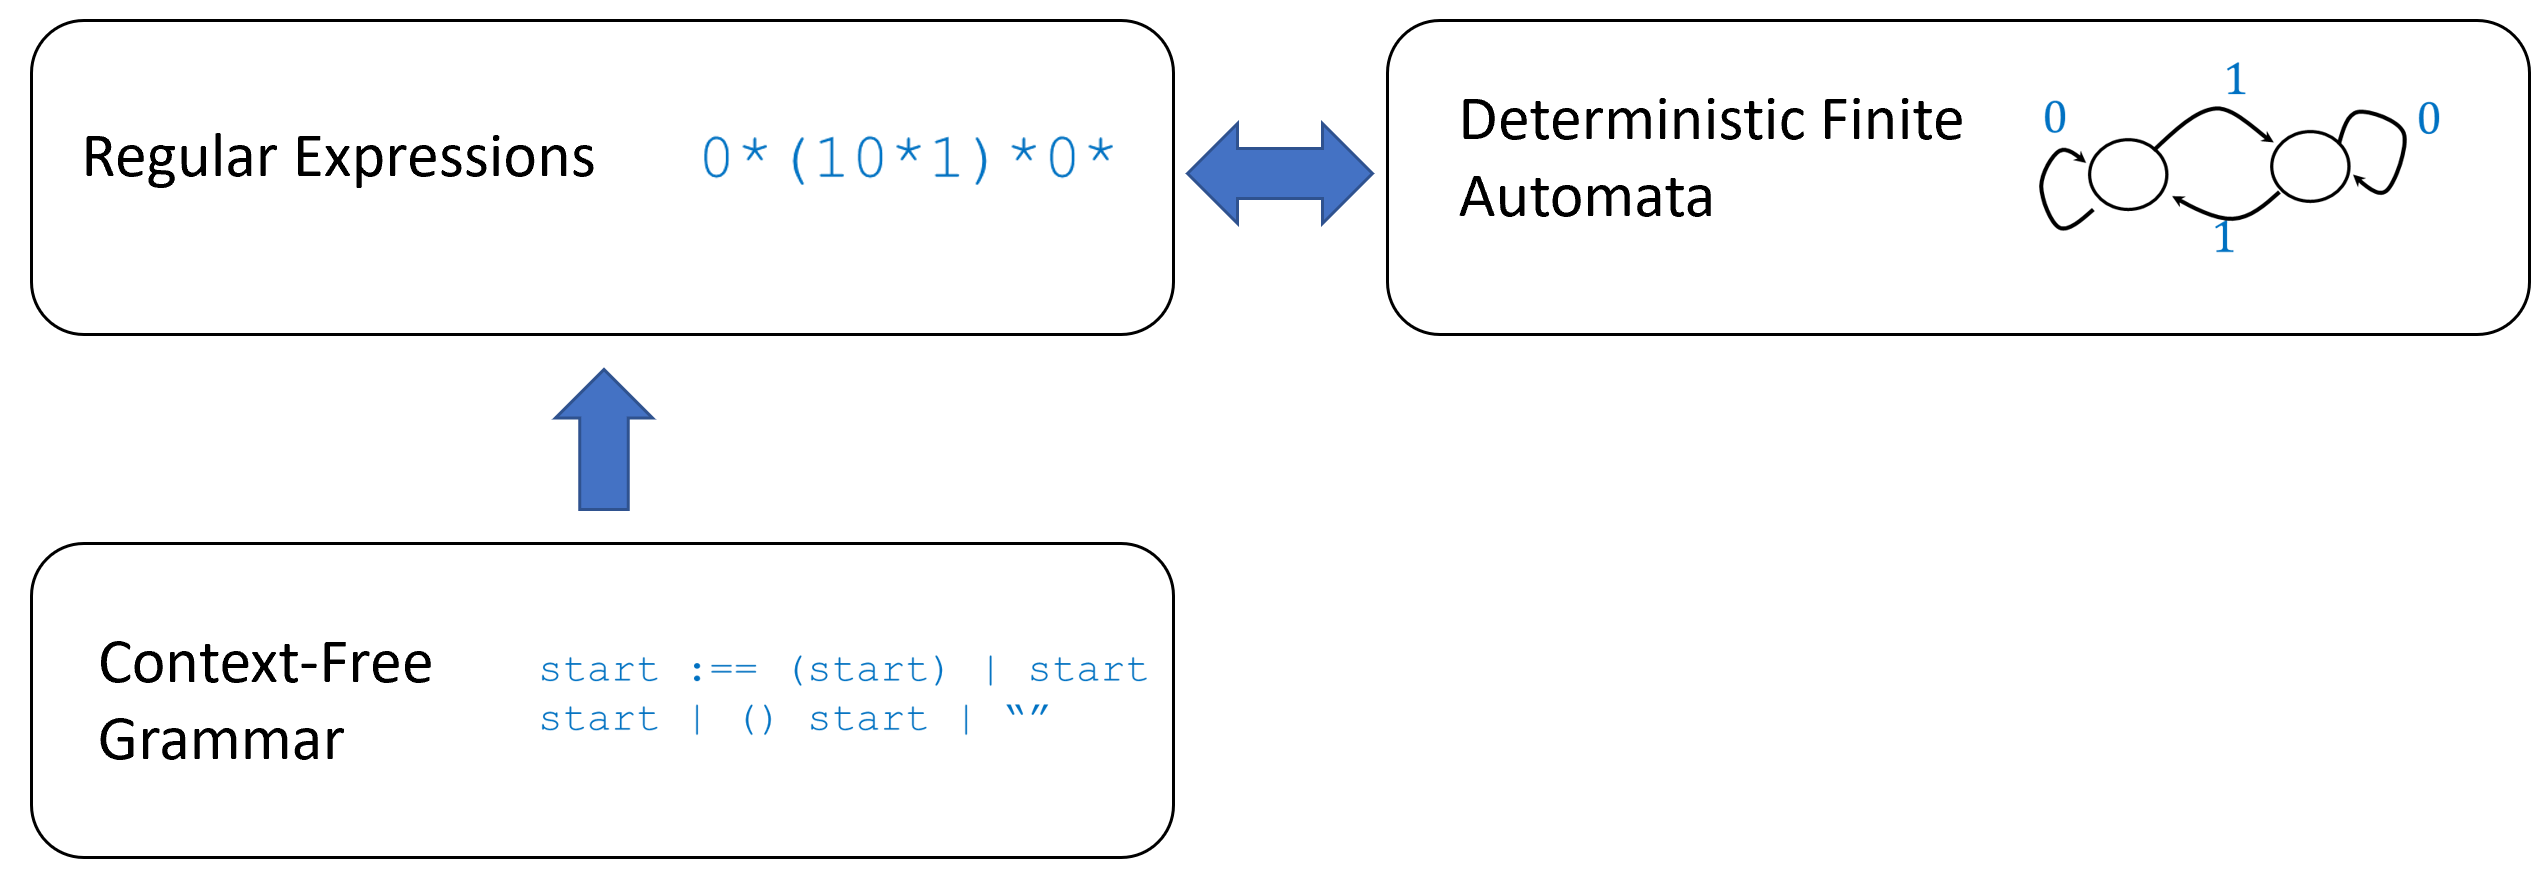
\includegraphics[width=\textwidth, height=0.25\paperheight, keepaspectratio]{../figure/restrictedoverview.png}
\caption{Some restricted computational models we study in this chapter.
We show two equivalent models of computation: regular expressions and
deterministic finite automata. We show a more powerful model:
context-free grammars. We also present tools to demonstrate that some
functions \emph{can not} be computed in these models.}
\label{restrictedmodelsoverviewfig}
\end{figure}

\section{Turing completeness as a bug}\label{Turing-completeness-as-a-}

We have seen that seemingly simple computational models or systems can
turn out to be Turing complete. The
\href{https://goo.gl/xRXq7p}{following webpage} lists several examples
of formalisms that ``accidentally'' turned out to Turing complete,
including supposedly limited languages such as the C preprocessor, CSS,
(certain variants of) SQL, sendmail configuration, as well as games such
as Minecraft, Super Mario, and the card game ``Magic: The Gathering''.
Turing completeness is not always a good thing, as it means that such
formalisms can give rise to arbitrarily complex behavior. For example,
the postscript format (a precursor of PDF) is a Turing-complete
programming language meant to describe documents for printing. The
expressive power of postscript can allow for short descriptions of very
complex images, but it also gave rise to some nasty surprises, such as
the attacks described in
\href{http://hacking-printers.net/wiki/index.php/PostScript}{this page}
ranging from using infinite loops as a denial of service attack, to
accessing the printer's file system.

\hypertarget{ethereum}{}
\begin{example}[The DAO Hack] \label[example]{ethereum}

An interesting recent example of the pitfalls of Turing-completeness
arose in the context of the cryptocurrency
\href{https://www.ethereum.org/}{Ethereum}. The distinguishing feature
of this currency is the ability to design ``smart contracts'' using an
expressive (and in particular Turing-complete) programming language. In
our current ``human operated'' economy, Alice and Bob might sign a
contract to agree that if condition X happens then they will jointly
invest in Charlie's company. Ethereum allows Alice and Bob to create a
joint venture where Alice and Bob pool their funds together into an
account that will be governed by some program \(P\) that decides under
what conditions it disburses funds from it. For example, one could
imagine a piece of code that interacts between Alice, Bob, and some
program running on Bob's car that allows Alice to rent out Bob's car
without any human intervention or overhead.

Specifically Ethereum uses the Turing-complete programming language
\href{https://solidity.readthedocs.io/en/develop/index.html}{solidity}
which has a syntax similar to JavaScript. The flagship of Ethereum was
an experiment known as The ``Decentralized Autonomous Organization'' or
\href{https://goo.gl/NegW77}{The DAO}. The idea was to create a smart
contract that would create an autonomously run decentralized venture
capital fund, without human managers, where shareholders could decide on
investment opportunities. The DAO was at the time the biggest
crowdfunding success in history. At its height the DAO was worth 150
million dollars, which was more than ten percent of the total Ethereum
market. Investing in the DAO (or entering any other ``smart contract'')
amounts to providing your funds to be run by a computer program. i.e.,
``code is law'', or to use the words the DAO described itself:
\emph{``The DAO is borne from immutable, unstoppable, and irrefutable
computer code''}. Unfortunately, it turns out that (as we saw in
\cref{chapcomputable}) understanding the behavior of computer programs
is quite a hard thing to do. A hacker (or perhaps, some would say, a
savvy investor) was able to fashion an input that caused the DAO code to
enter into an infinite recursive loop in which it continuously
transferred funds into the hacker's account, thereby
\href{https://www.bloomberg.com/features/2017-the-ether-thief/}{cleaning
out about 60 million dollars} out of the DAO. While this transaction was
``legal'' in the sense that it complied with the code of the smart
contract, it was obviously not what the humans who wrote this code had
in mind. The Ethereum community struggled with the response to this
attack. Some tried to the ``Robin Hood'' approach of using the same
loophole to drain the DAO funds into a secure account, but it only had
limited success. Eventually, the Ethereum community decided that the
code can be mutable, stoppable, and refutable. Specifically, the
Ethereum maintainers and miners agreed on a ``hard fork'' (also known as
a ``bailout'') to revert history to before the hacker's transaction
occurred. Some community members strongly opposed this decision, and so
an alternative currency called
\href{https://ethereumclassic.github.io/}{Ethereum Classic} was created
that preserved the original history.

\end{example}

\section{Regular expressions}\label{Regular-expressions}

\emph{Searching} for a piece of text is a common task in computing. At
its heart, the \emph{search problem} is quite simple. We have a
collection \(X = \{ x_0, \ldots, x_k \}\) of strings (e.g., files on a
hard-drive, or student records in a database), and the user wants to
find out the subset of all the \(x \in X\) that are \emph{matched} by
some pattern (e.g., all files whose names end with the string
\texttt{.txt}). In full generality, we can allow the user to specify the
pattern by specifying a (computable) \emph{function}
\(F:\{0,1\}^* \rightarrow \{0,1\}\), where \(F(x)=1\) corresponds to the
pattern matching \(x\). That is, the user provides a \emph{program}
\(P\) in some Turing-complete programming language such as
\emph{Python}, and the system will return all the \(x \in X\) such that
\(P(x)=1\). For example, one could search for all text files that
contain the string \texttt{important document} or perhaps (letting \(P\)
correspond to a neural-network based classifier) all images that contain
a cat. However, we don't want our system to get into an infinite loop
just trying to evaluate the program \(P\)!

Because the Halting problem for Turing-complete computational models is
uncomputable, we cannot in general verify that a given program \(P\)
will halt on a given input. For this reason, typical systems for
searching files or databases do \emph{not} allow users to specify the
patterns using full-fledged programming languages. Rather, such systems
use \emph{restricted computational models} that on the one hand are
\emph{rich enough} to capture many of the queries needed in practice
(e.g., all filenames ending with \texttt{.txt}, or all phone numbers of
the form \texttt{(617) xxx-xxxx}), but on the other hand are
\emph{restricted} enough so that they cannot result in an infinite loop.

One of the most popular such computational models is
\href{https://goo.gl/2vTAFU}{regular expressions}. If you ever used an
advanced text editor, a command line shell, or have done any kind of
manipulation of text files, then you have probably come across regular
expressions.

A \emph{regular expression} over some alphabet \(\Sigma\) is obtained by
combining elements of \(\Sigma\) with the operation of concatenation, as
well as \(|\) (corresponding to \emph{or}) and \(*\) (corresponding to
repetition zero or more times). (Common implementations of regular
expressions in programming languages and shells typically include some
extra operations on top of \(|\) and \(*\), but these operations can be
implemented as ``syntactic sugar'' using the operators \(|\) and \(*\).)
For example, the following regular expression over the alphabet
\(\{0,1\}\) corresponds to the set of all strings \(x\in \{0,1\}^*\)
where every digit is repeated at least twice: \[
(00(0^*)|11(1^*))^* \;.
\]

The following regular expression over the alphabet
\(\{ a,\ldots,z,0,\ldots,9 \}\) corresponds to the set of all strings
that consist of a sequence of one or more of the letters \(a\)-\(d\)
followed by a sequence of one or more digits (without a leading zero):

\[
(a|b|c|d)(a|b|c|d)^*(1|2|3|4|5|6|7|8|9)(0|1|2|3|4|5|6|7|8|9)^* \;. \label{regexpeq}
\]

Formally, regular expressions are defined by the following recursive
definition:

\hypertarget{regexp}{}
\begin{definition}[Regular expression] \label[definition]{regexp}

A \emph{regular expression} \(e\) over an alphabet \(\Sigma\) is a
string over
\(\Sigma \cup \{ (,),|,*,\emptyset, \ensuremath{\text{\texttt{""}}} \}\)
that has one of the following forms:

\begin{enumerate}
\def\labelenumi{\arabic{enumi}.}
\item
  \(e = \sigma\) where \(\sigma \in \Sigma\)
\item
  \(e = (e' | e'')\) where \(e', e''\) are regular expressions.
\item
  \(e = (e')(e'')\) where \(e',e''\) are regular expressions. (We often
  drop the parentheses when there is no danger of confusion and so write
  this as \(e' \; e''\).)
\item
  \(e = (e')^*\) where \(e'\) is a regular expression.
\end{enumerate}

Finally we also allow the following ``edge cases'': \(e = \emptyset\)
and \(e = \ensuremath{\text{\texttt{""}}}\). These are the regular
expressions corresponding to accepting no strings, and accepting only
the empty string respectively.

\end{definition}

We will drop parenthesis when they can be inferred from the context. We
also use the convention that OR and concatenation are left-associative,
and give higher precedence to \(*\), then concatenation, and then OR.
Thus for example we write \(00^*|11\) instead of
\(((0)(0^*))|((1)(1))\).

Every regular expression \(e\) corresponds to a function
\(\Phi_{e}:\Sigma^* \rightarrow \{0,1\}\) where \(\Phi_{e}(x)=1\) if
\(x\) \emph{matches} the regular expression. For example, if
\(e = (00|11)^*\) then \(\Phi_e(110011)=1\) but \(\Phi_e(101)=0\) (can
you see why?).

\begin{pause} \label[pause]{The-formal-definition-of-}

The formal definition of \(\Phi_{e}\) is one of those definitions that
is more cumbersome to write than to grasp. Thus it might be easier for
you to first work it out on your own and then check that your definition
matches what is written below.

\end{pause}

\hypertarget{matchingregexpdef}{}
\begin{definition}[Matching a regular expression] \label[definition]{matchingregexpdef}

Let \(e\) be a regular expression over the alphabet \(\Sigma\). The
function \(\Phi_{e}:\Sigma^* \rightarrow \{0,1\}\) is defined as
follows:

\begin{enumerate}
\def\labelenumi{\arabic{enumi}.}
\item
  If \(e = \sigma\) then \(\Phi_{e}(x)=1\) iff \(x=\sigma\).
\item
  If \(e = (e' | e'')\) then
  \(\Phi_{e}(x) = \Phi_{e'}(x) \vee \Phi_{e''}(x)\) where \(\vee\) is
  the OR operator.
\item
  If \(e = (e')(e'')\) then \(\Phi_{e}(x) = 1\) iff there is some
  \(x',x'' \in \Sigma^*\) such that \(x\) is the concatenation of \(x'\)
  and \(x''\) and \(\Phi_{e'}(x')=\Phi_{e''}(x'')=1\).
\item
  If \(e= (e')*\) then \(\Phi_{e}(x)=1\) iff there are is \(k\in \N\)
  and some \(x_0,\ldots,x_{k-1} \in \Sigma^*\) such that \(x\) is the
  concatenation \(x_0 \cdots x_{k-1}\) and \(\Phi_{e'}(x_i)=1\) for
  every \(i\in [k]\).
\item
  Finally, for the edge cases \(\Phi_{\emptyset}\) is the constant zero
  function, and \(\Phi_{\ensuremath{\text{\texttt{""}}}}\) is the
  function that only outputs \(1\) on the empty string
  \(\ensuremath{\text{\texttt{""}}}\).
\end{enumerate}

We say that a regular expression \(e\) over \(\Sigma\) \emph{matches} a
string \(x \in \Sigma^*\) if \(\Phi_{e}(x)=1\). We say that a function
\(F:\Sigma^* \rightarrow \{0,1\}\) is \emph{regular} if \(F=\Phi_{e}\)
for some regular expression \(e\).\footnote{We use \emph{function
  notation} in this book, but other texts often use the notion of
  \emph{languages}, which are sets of strings. In that notation a
  language \(L \subseteq \Sigma^*\) is called \emph{regular} if and only
  if the corresponding function \(F_L\) is regular, where
  \(F_L:\Sigma^* \rightarrow \{0,1\}\) is the function that outputs
  \(1\) on \(x\) iff \(x\in L\).}

\end{definition}

\begin{pause} \label[pause]{The-definitions-above-are}

The definitions above are not inherently difficult, but are a bit
cumbersome. So you should pause here and go over it again until you
understand why it corresponds to our intuitive notion of regular
expressions. This is important not just for understanding regular
expressions themselves (which are used time and again in a great many
applications) but also for getting better at understanding recursive
definitions in general.

\end{pause}

\hypertarget{regularexpmatching}{}
\begin{example}[A regular function] \label[example]{regularexpmatching}

Let \(\Sigma=\{ a,b,c,d,0,1,2,3,4,5,6,7,8,9 \}\) and
\(F:\Sigma^* \rightarrow \{0,1\}\) be the function such that \(F(x)\)
outputs \(1\) iff \(x\) consists of one or more of the letters
\(a\)-\(d\) followed by a sequence of one or more digits (without a
leading zero). Then \(F\) is a regular function, since \(F=\Phi_e\)
where
\[e = (a|b|c|d)(a|b|c|d)^*(0|1|2|3|4|5|6|7|8|9)(0|1|2|3|4|5|6|7|8|9)^*\]
is the expression we saw in \eqref{regexpeq}.

If we wanted to verify, for example, that \(\Phi_e(abc12078)=1\), we can
do so by noticing that the expression \((a|b|c|d)\) matches the string
\(a\), \((a|b|c|d)^*\) matches \(bc\), \((0|1|2|3|4|5|6|7|8|9)\) matches
the string \(1\), and the expression \((0|1|2|3|4|5|6|7|8|9)^*\) matches
the string \(2078\). Each one of those boils down to a simpler
expression. For example, the expression \((a|b|c|d)^*\) matches the
string \(bc\) because both of the one-character strings \(b\) and \(c\)
are matched by the expression \(a|b|c|d\).

\end{example}

Regular expression can be defined over any finite alphabet \(\Sigma\),
but as usual, we will focus our attention on the \emph{binary case},
where \(\Sigma = \{0,1\}\). Most (if not all) of the theoretical and
practical general insights about regular expressions can be gleaned from
studying the binary case.

We can think of regular expressions as a type of ``programming
language''. That is, we can think of a regular expression \(e\) over the
alphabet \(\Sigma\) as a program that computes the function
\(\Phi_{e}:\Sigma^* \rightarrow \{0,1\}\). (You can also think of
regular expressions as \emph{generative models}, since you can think of
them as giving a recipe how to generate strings that match them.) This
``regular expression programming language'' is simpler than general
programming languages, in the sense that for every regular expression
\(e\), the function \(\Phi_e\) is computable (and so in particular can
be evaluated by an always-halting Turing machine).

\hypertarget{regularexphalt}{}
\begin{theorem}[Regular expression always halt] \label[theorem]{regularexphalt}

For every regular expression \(e\) over \(\{0,1\}\), the function
\(\Phi_e:\{0,1\}^* \rightarrow \{0,1\}\) is computable.

That is, there is a Turing machine \(M\) such that for every
\(x\in \{0,1\}^*\), on input \(x\), \(M\) halts with the output
\(\Phi_e(x)\).

\end{theorem}

We state \cref{regularexphalt} for regular expressions over the binary
alphabet \(\{0,1\}\), but it generalizes to any finite alphabet
\(\Sigma\).

\begin{proofidea} \label[proofidea]{The-proof-relies-on-the-o}

The proof relies on the observation that \cref{matchingregexpdef}
actually specifies a recursive algorithm for \emph{computing}
\(\Phi_{e}\). Specifically, each one of our operations -concatenation,
OR, and star- can be thought of as reducing the task of testing whether
an expression \(e\) matches a string \(x\) to testing whether some
sub-expressions of \(e\) match substrings of \(x\). Since these
sub-expressions are always shorter than the original expression, this
yields a recursive algorithm for checking if \(e\) matches \(x\) which
will eventually terminate at the base cases of the expressions that
correspond to a single symbol or the empty string.

\end{proofidea}

\begin{proof}[Proof of \cref{regularexphalt}] \label[proof]{crefmatchingregexpdef-giv}

\cref{matchingregexpdef} gives a way of recursively computing
\(\Phi_{e}\). The key observation is that in our recursive definition of
regular expressions, whenever \(e\) is made up of one or two expressions
\(e',e''\) then these two regular expressions are \emph{smaller} than
\(e\), and eventually (when they have size \(1\)) then they must
correspond to the non-recursive case of a single alphabet symbol.

Therefore, we can prove the theorem by induction over the length \(m\)
of \(e\) (i.e., the number of symbols in the string \(e\), also denoted
as \(|e|\)). For \(m=1\), \(e\) is either a single alphabet symbol,
\(\ensuremath{\text{\texttt{""}}}\) or \(\emptyset\), and so computing
the function \(\Phi_{e}\) is straightforward. In the general case, for
\(m=|e|\) we assume by the induction hypothesis that we have proven the
theorem for all expressions of length smaller than \(m\). Now, such an
expression of length larger than one can obtained through one of three
cases: OR, concatenation, or star operations. We now show that
\(\Phi_{e}\) will be computable in all these cases:

\textbf{Case 1:} \(e = (e' | e'')\) where \(e', e''\) are shorter
regular expressions.

In this case by the inductive hypothesis we can compute \(\Phi_{e'}\)
and \(\Phi_{e''}\) and so can compute \(\Phi_{e}(x)\) as
\(\Phi_{e'}(x) \vee \Phi_{e''}(x)\) (where \(\vee\) is the OR operator).

\textbf{Case 2:} \(e = (e')(e'')\) where \(e',e''\) are regular
expressions.

In this case by the inductive hypothesis we can compute \(\Phi_{e'}\)
and \(\Phi_{e''}\) and so can compute \(\Phi_{e}(x)\) as

\[\bigvee_{i=0}^{|x|-1}(\Phi_{e'}(x_0\cdots x_{i-1})  \wedge \Phi_{e''}(x_i \cdots x_{|x|-1}))\]

where \(\wedge\) is the AND operator and for \(i<j\),
\(x_j \cdots x_{i}\) refers to the empty string.

\textbf{Case 3:} \(e = (e')*\) where \(e'\) is a regular expression.

In this case by the inductive hypothesis we can compute \(\Phi_{e'}\)
and so we can compute \(\Phi_{e}(x)\) by enumerating over all \(k\) from
\(1\) to \(|x|\), and all ways to write \(x\) as the concatenation of
\(k\) nonempty strings \(x_0 \cdots x_{k-1}\) (we can do so by
enumerating over all possible \(k-1\) positions in which one string
stops and the other begins). If for one of those partitions,
\(\Phi_{e'}(x_0)=\cdots = \Phi_{e'}(x_{k-1})=1\) then we output \(1\).
Otherwise we output \(0\). We can restrict attention to partitions of
\(x\) as \(x=x_0 \cdots x_{k-1}\) where all the \(x_i\)'s are nonempty
since if some of the \(x_i\)'s are empty we can simply drop them and
still be left with a valid partition.

These three cases exhaust all the possibilities for an expression of
length larger than one, and hence this completes the proof.

\end{proof}

\section{Deterministic finite automata, and efficient matching of
regular expressions (optional)}\label{Deterministic-finite-auto}

The proof of \cref{regularexphalt} gives a recursive algorithm to
evaluate whether a given string matches or not a regular expression. But
it is not a very efficient algorithm.

However, it turns out that there is a much more efficient algorithm that
can match regular expressions in \emph{linear} (i.e., \(O(n)\)) time.
Since we have not yet covered the topics of time and space complexity,
we describe this algorithm in high level terms, without making the
computational model precise, using the colloquial notion of \(O(n)\)
running time as is used in introduction to programming courses and
whiteboard coding interviews. We will see a formal definition of time
complexity in \cref{chapmodelruntime}.

\hypertarget{reglintimethm}{}
\begin{theorem}[Matching regular expressions in linear time] \label[theorem]{reglintimethm}

Let \(e\) be a regular expression. Then there is an \(O(n)\) time
algorithm that computes \(\Phi_{e}\).

\end{theorem}

The implicit constant in the \(O(n)\) term of \cref{reglintimethm}
depends on the expression \(e\). Thus, another way to state
\cref{reglintimethm} is that for every expression \(e\), there is some
constant \(c\) and an algorithm \(A\) that computes \(\Phi_e\) on
\(n\)-bit inputs using at most \(c\cdot n\) steps. This makes sense,
since in practice we often want to compute \(\Phi_e(x)\) for a small
regular expression \(e\) and a large document \(x\).
\cref{reglintimethm} tells us that we can do so with running time that
scales linearly with the size of the document, even if it has
(potentially) worse dependence on the size of the regular expression.

\begin{proofidea} \label[proofidea]{The-idea-is-to-define-a-m}

The idea is to define a more efficient recursive algorithm, that
determines whether \(e\) matches a string \(x\in \{0,1\}^n\) by reducing
this task to determining whether a related expression \(e'\) matches
\(x_0,\ldots,x_{n-1}\). This will result in an expression for the
running time of the form \(T(n) = T(n-1) + O(1)\) which solves to
\(T(n)=O(n)\).

\end{proofidea}

\begin{proof}[Proof of \cref{reglintimethm}] \label[proof]{The-central-definition-fo}

The central definition for this proof is the notion of a
\emph{restriction} of a regular expression. The idea is that for every
regular expression \(e\) and symbol \(\sigma\) in its alphabet, it is
possible to define a regular expression \(e[\sigma]\) such that
\(e[\sigma]\) matches a string \(x\) if and only if \(e\) matches the
string \(x\sigma\). For example, if \(e\) is the regular expression
\(01|(01)*(01)\) (i.e., one or more occurrences of \(01\)) then \(e[1]\)
is equal to \(0|(01)*0\) and \(e[0]\) will be \(\emptyset\). (Can you
see why?)

For simplicity, from now on we fix our attention to the case that the
alphabet \(\Sigma\) is \(\{0,1\}\). Given a regular expression \(e\) and
\(\sigma\in \{0,1\}\), we can compute \(e[\sigma]\) recursively as
follows:

\begin{enumerate}
\def\labelenumi{\arabic{enumi}.}
\item
  If \(e\) consists of a single symbol (i.e.~\(e=\tau\) for
  \(\tau \in \{0,1\}\)) then
  \(e[\sigma]=\ensuremath{\text{\texttt{""}}}\) if \(\tau=\sigma\) and
  \(e[\sigma]=\emptyset\) otherwise.
\item
  If \(e = e' | e''\) then \(e[\sigma] = e'[\sigma] | e''[\sigma]\).
\item
  If \(e = e' \; e''\) then \(e[\sigma] = e' \; e''[\sigma]\) if \(e''\)
  can not match the empty string. Otherwise,
  \(e[\sigma] = e' \; e''[\sigma] \; | \; e'[\sigma]\)
\item
  If \(e = (e')^*\) then \(e[\sigma] = (e')^*(e'[\sigma])\).
\item
  If \(e = \ensuremath{\text{\texttt{""}}}\) or \(e= \emptyset\) then
  \(e[\sigma] = \emptyset\).
\end{enumerate}

By checking all these cases, one can verify that it is indeed the case
that for every regular expression \(e\), \(\sigma \in \{0,1\}\) and
\(x\in \{0,1\}^*\), \(e[\sigma]\) matches \(x\) if and only if \(e\)
matches \(x\sigma\). We let \(C(\ell)\) denote the time to compute
\(e[\sigma]\) for regular expressions of length at most \(\ell\). The
value \(C(\ell)\) can be shown to be polynomial in \(\ell\), though this
is not important for this theorem, since we only care about the
dependence of the time to compute \(\Phi_e(x)\) on the length of \(x\)
and not about the dependence of this time on the length of \(e\).

Using this notion of restriction, we can define the following recursive
algorithm for regular expression matching:

\hypertarget{regexpmatchlinearalg}{}
\begin{algorithm}[Regular expression matching in linear time] \label[algorithm]{regexpmatchlinearalg}~ \\ \noindent

\textbf{Input:} Regular expression \(e\) over \(\{0,1\}\) and
\(x\in \{0,1\}^n\) for \(n\in \N\).

\textbf{Goal:} Compute \(\Phi_e(x)\)

\textbf{Operation:}

\begin{enumerate}
\def\labelenumi{\arabic{enumi}.}
\item
  If \(x=\ensuremath{\text{\texttt{""}}}\) then return \(1\) if and only
  if \(\Phi_e(\ensuremath{\text{\texttt{""}}})=1\). (This can be either
  computed directly or using the algorithm of \cref{regularexphalt} in
  time which is a constant depending only on the regular expression
  \(e\).)
\item
  Otherwise, compute \(\Phi_{e[x_{n-1}]}(x_0\cdots x_{n-1})\)
  recursively and output the result.
\end{enumerate}

\end{algorithm}

By the definition of a restriction, for every \(\sigma\in \{0,1\}\) and
\(x'\in \{0,1\}^*\), the expression \(e\) matches \(x'\sigma\) if and
only if \(e[\sigma]\) matches \(x'\). Hence for every \(e\) and
\(x\in \{0,1\}^n\), \(\Phi_{e[x_{n-1}]}(x_0\cdots x_{n-2}) = \Phi_e(x)\)
and \cref{regexpmatchlinearalg} does return the correct answer. The only
remaining task is to analyze its \emph{running time}.

\cref{regexpmatchlinearalg} is a recursive algorithm that on input an
expression \(e\) and a string \(x\in \{0,1\}^n\), does some constant
time computation and then calls itself on input some expression \(e'\)
and a string \(x\) of length \(n-1\). It will terminate after \(n\)
steps when it reaches a string of length \(0\). So, to calculate the
running time of \cref{regexpmatchlinearalg} we need to analyze the cost
of each step.

Specifically, the running time \(T(e,n)\) that it takes for
\cref{regexpmatchlinearalg} to compute \(\Phi_e\) for inputs of length
\(n\) satisfies the recursive equation:

\[T(e,n) = \max \{ T(e[0],n-1) , T(e[1],n-1)  \} + C(|e|)
\label{matchregexprecursion} \]

where \(C(\ell)\), as before, denotes the time to compute \(e[\sigma]\)
for expressions \(e\) of length at most \(\ell\). (In the base case
\(n=0\), \(T(e,0)\) is equal to some constant depending only on \(e\).)

To get some intuition for the expression \cref{matchregexprecursion},
let us open up the recursion for one level, writing \(T(e,n)\) as

\[\begin{aligned}T(e,n) &= \max \{ T(e[0][0],n-2) + C(|e[0]|), \\ &T(e[0][1],n-2) + C(|e[0]|), \\
&T(e[1][0],n-2) + C(|e[1]|),  \\
&T(e[1][1],n-2) + C(|e[1]|) \} + C(|e|)\;.\end{aligned}\]

Continuing this way, we can see that
\(T(e,n) \leq n \cdot C(\ell) + O(1)\) where \(\ell\) is the largest
length of any expression \(e'\) that we encounter along the way.
Therefore, the following claim suffices to show that
\cref{regexpmatchlinearalg} runs in linear time:

\textbf{Claim:} Let \(e\) be a regular expression over \(\{0,1\}\), then
there is some constant \(c\) such that for every string
\(\alpha\in \{0,1\}^*\), if we restrict \(e\) to \(\alpha_0\), and then
to \(\alpha_1\) and so on and so forth, the resulting expression has
length at most \(c\).

\begin{quote} \label[quote]{Proof-of-claim-For-a-regu}

\textbf{Proof of claim:} For a regular expression \(e\) over \(\{0,1\}\)
and \(\alpha\in \{0,1\}^m\), we denote by \(e[\alpha]\) the expression
\(e[\alpha_0][\alpha_1]\cdots [\alpha_{m-1}]\) obtained by restricting
\(e\) to \(\alpha_0\) and then to \(\alpha_1\) and so on. We let
\(S(e) = \{ e[\alpha] | \alpha \in \{0,1\}^* \}\). We will prove the
claim by showing that for every \(e\), the set \(S(e)\) is finite, and
hence so is the number \(c(e)\) which is the maximum length of \(e'\)
for \(e'\in S(e)\).

We prove this by induction on the structure of \(e\). If \(e\) is a
symbol, the empty string, or the empty set, then this is straightforward
to show as the most expressions \(S(e)\) can contain are the expression
itself, \(\ensuremath{\text{\texttt{""}}}\), and \(\emptyset\).
Otherwise we split to the two cases \textbf{(i)} \(e = e'^*\) and
\textbf{(ii)} \(e = e'e''\), where \(e',e''\) are smaller expressions
(and hence by the induction hypothesis \(S(e')\) and \(S(e'')\) are
finite). In the case \textbf{(i)}, if \(e = (e')^*\) then \(e[\alpha]\)
is either equal to \((e')^* e'[\alpha]\) or it is simply the empty set
if \(e'[\alpha]=\emptyset\). Since \(e'[\alpha]\) is in the set
\(S(e')\), the number of distinct expressions in \(S(e)\) is at most
\(|S(e')|+1\). In the case \textbf{(ii)}, if \(e = e' e''\) then all the
restrictions of \(e\) to strings \(\alpha\) will either have the form
\(e' e''[\alpha]\) or the form \(e' e''[\alpha] | e'[\alpha']\) where
\(\alpha'\) is some string such that \(\alpha = \alpha' \alpha''\) and
\(e[\alpha'']\) matches the empty string. Since
\(e''[\alpha] \in S(e'')\) and \(e'[\alpha'] \in S(e')\), the number of
the possible distinct expressions of the form \(e[\alpha]\) is at most
\(|S(e'')| + |S(e'')|\cdot |S(e')|\). This completes the proof of the
claim.

\end{quote}

The bottom line is that while running \cref{regexpmatchlinearalg} on a
regular expression \(e\), all the expressions we ever encounter are in
the finite set \(S(e)\), no matter how large the input \(x\) is, and so
the running time of \cref{regexpmatchlinearalg} satisfies the equation
\(T(n) = T(n-1) + C'\) for some constant \(C'\) depending on \(e\). This
solves to \(O(n)\) where the implicit constant in the Oh notation can
(and will) depend on \(e\) but crucially, not on the length of the input
\(x\).

\end{proof}

\subsection{Matching regular expressions using constant
memory}\label{Matching-regular-expressi}

\cref{reglintimethm} is already quite impressive, but we can do even
better. Specifically, no matter how long the string \(x\) is, we can
compute \(\Phi_e(x)\) by maintaining only a constant amount of memory
and moreover making a \emph{single pass} over \(x\). That is, the
algorithm will scan the input \(x\) once from start to finish, and then
determine whether or not \(x\) is matched by the expression \(e\). This
is important in the common case of trying to match a short regular
expression over a huge file or document that might not even fit in our
computer's memory. A single-pass constant-memory algorithm is also known
as a \href{https://goo.gl/SG6DS7}{deterministic finite automaton (DFA)}
(see \cref{secdfa}). There is a beautiful theory on the properties of
DFA's and their connections with regular expressions. In particular, as
we'll see in \cref{dfaregequivthm}, a function is regular \emph{if and
only if} it can be computed by a DFA. We start with showing the ``only
if'' direction:

\hypertarget{DFAforREGthm}{}
\begin{theorem}[DFA for regular expression matching] \label[theorem]{DFAforREGthm}

Let \(e\) be a regular expression. Then there is an algorithm that on
input \(x\in \{0,1\}^*\) computes \(\Phi_e(x)\) while making a single
pass over \(x\) and maintaining a constant amount of memory.

\end{theorem}

\begin{proofidea} \label[proofidea]{The-idea-is-to-replace-th}

The idea is to replace the recursive algorithm of
\cref{regexpmatchlinearalg} with a \href{https://goo.gl/kgLdX1}{dynamic
program}, using the technique of
\href{https://en.wikipedia.org/wiki/Memoization}{memoization}. If you
haven't taken yet an algorithms course, you might not know these
techniques. This is OK; while this more efficient algorithm is crucial
for the many practical applications of regular expressions, it is not of
great importance for this book.

\end{proofidea}

\begin{proof}[Proof of \cref{DFAforREGthm}] \label[proof]{We-will-replace-the-recur}

We will replace the recursive \cref{regexpmatchlinearalg} with the
following iterative algorithm:

\hypertarget{iterregexpmatchlinearalg}{}
\begin{algorithm}[Constant memory regular expression matching] \label[algorithm]{iterregexpmatchlinearalg}~ \\ \noindent

\textbf{Input:} Regular expression \(e\) over \(\{0,1\}\), string
\(x\in \{0,1\}^n\).

\textbf{Goals:} Compute \(\Phi_e(x)\).

\textbf{Operation:}

\begin{enumerate}
\def\labelenumi{\arabic{enumi}.}
\item
  Let \(S = S(e)\) be the set \(\{ e[\alpha] | \alpha\in \{0,1\}^* \}\)
  as defined in the proof of \cref{reglintimethm}. Note that \(S\) is
  finite and by definition, for every \(e' \in S\) and
  \(\sigma \in \{0,1\}\), \(e'[\sigma]\) is in \(S\) as well.
\item
  Define a Boolean variable \(v_{e'}\) for every \(e' \in S\). Initially
  we set \(v_{e'}=1\) if and only if \(e'\) matches the empty string.
\item
  For \(i=0,\ldots,n-1\) do the following:

  \begin{enumerate}
  \def\labelenumii{\alph{enumii}.}
  \item
    \emph{Copy the variables \(\{ v_{e'} \}\) to temporary variables:}
    For every \(e' \in S\), we set \(temp_{e'} = v_{e'}\).
  \item
    \emph{Update the variables \(\{ v_{e'} \}\) based on the \(i\)-th
    bit of \(x\):} Let \(\sigma = x_i\) and set
    \(v_{e'} = temp_{e'[\sigma]}\) for every \(e' \in S\).
  \end{enumerate}
\item
  Output \(v_{e}\).
\end{enumerate}

\end{algorithm}

\cref{iterregexpmatchlinearalg} maintains the invariant that at the end
of step \(i\), for every \(e' \in S\), the variable \(v_{e'}\) is equal
if and only if \(e'\) matches the string \(x_0\cdots x_{i-1}\). In
particular, at the very end, \(v_{e}\) is equal to \(1\) if and only if
\(e\) matches the full string \(x_0 \cdots x_{n-1}\).
\cref{iterregexpmatchlinearalg} only maintains a constant number of
variables (as \(S\) is finite), and that it proceeds in one linear scan
over the input, and so this proves the theorem.

\end{proof}

\subsection{Deterministic Finite Automata}\label{secdfa}

In Computer Science, a single-pass constant-memory algorithm is also
known as a \emph{Deterministic Finite Automaton} or \emph{DFA} (another
name for DFA's is a \emph{finite state machine}). That is, we can think
of such an algorithm as a ``machine'' that can be in one of \(C\)
states, for some constant \(C\). The machine starts in some initial
state, and then reads its input \(x\in \{0,1\}^*\) one bit at a time.
Whenever the machine reads a bit \(\sigma \in \{0,1\}\), it transitions
into a new state based on \(\sigma\) and its prior state. The output of
the machine is based on the final state. Every constant-memory one-pass
algorithm corresponds to such a machine. If an algorithm uses \(c\) bits
of memory, then the contents of its memory are a string of length \(c\).
Since there are \(2^c\) such strings, at any point in the execution,
such an algorithm can be in one of \(2^c\) states.

\hypertarget{DFAforparity}{}
\begin{example}[DFA for XOR] \label[example]{DFAforparity}

Here is a DFA for computing the function
\(\ensuremath{\mathit{XOR}}:\{0,1\}^* \rightarrow \{0,1\}\) that maps
\(x\) to \(\sum_{i\in [|x|]} x_i \mod 2\).

We will have two states: \(0\) and \(1\). The set of accepting states is
\(\{1 \}\), and if we are in a state \(v \in \{0,1\}\) and read the bit
\(\sigma\), we will transition to the state \(v\) if \(\sigma=0\) and to
the state \(1-v\) if \(\sigma = 1\). In other words, we transition to
the state \(v \oplus \sigma\). Hence we can think of this algorithm's
execution on input \(x\in \{0,1\}^n\) as follows:

\begin{itemize}
\item
  Let \(v_t\) be the state of the automaton at step \(t\). We initialize
  \(v_t=0\).
\item
  For every \(i\in [n]\), let \(v_i = v_{i+1} \oplus x_i\).
\item
  Output \(v_n\).
\end{itemize}

You can verify that the output of this algorithm is
\(x_0 \oplus x_1 \oplus \cdots \oplus x_{n-1} = \ensuremath{\mathit{XOR}}(x)\).
We can also describe this DFA graphically, see \cref{xorautomatonfig}.

\end{example}


\begin{marginfigure}
\centering
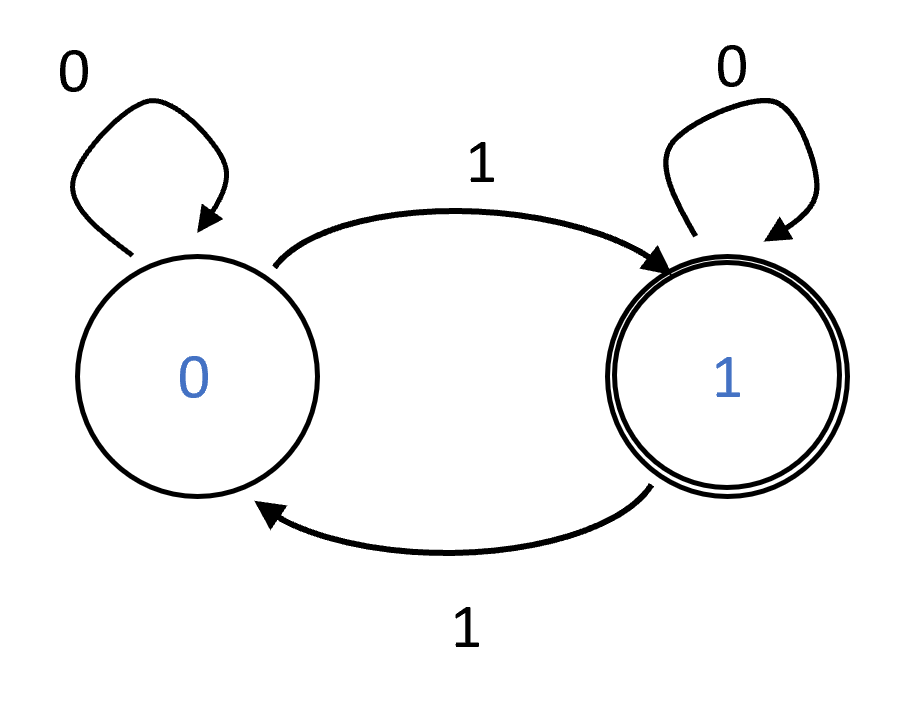
\includegraphics[width=\linewidth, height=1.5in, keepaspectratio]{../figure/xorautomaton.png}
\caption{A deterministic finite automaton that computes the
\(\ensuremath{\mathit{XOR}}\) function. It has two states \(0\) and
\(1\), and when it observes \(\sigma\) it transitions from \(v\) to
\(v \oplus \sigma\).}
\label{xorautomatonfig}
\end{marginfigure}

The formal definition of a DFA is the following:

\hypertarget{DFAdef}{}
\begin{definition}[Deterministic Finite Automaton] \label[definition]{DFAdef}

A deterministic finite automaton (DFA) with \(C\) states over
\(\{0,1\}\) is a pair \((T,\mathcal{S})\) with
\(T:[C]\times \{0,1\} \rightarrow [C]\) and
\(\mathcal{S} \subseteq [C]\). The function \(T\) is known as the
\emph{transition function} of the DFA and the set \(\mathcal{S}\) is
known as the set of \emph{accepting states}.

We say that \((T,\mathcal{S})\) \emph{computes} a function
\(F:\{0,1\}^* \rightarrow \{0,1\}\) if for every \(n\in\N\) and
\(x\in \{0,1\}^n\), if we define \(v_0=0\) and \(v_{i+1} = T(v_i,x_i)\)
for every \(i\in [n]\), then \[
v_n \in \mathcal{S}   \Leftrightarrow F(x)=1
\]

\end{definition}

\begin{pause} \label[pause]{Our-treatment-of-automata}

Our treatment of automata in this book is quite brief. If you find this
definition confusing, there are plenty of resources that help you get
more comfortable with DFA's. In particular, Chapter 1 of Sipser's book
\cite{SipserBook} contains an excellent exposition of this material.
There are also many websites with online simulators for automata, as
well as translators from regular expressions to automata and vice versa
(see for example
\href{http://ivanzuzak.info/noam/webapps/fsm2regex/}{here} and
\href{https://cyberzhg.github.io/toolbox/nfa2dfa}{here}).

Sipser defines a DFAs as a five-tuple \((Q,\Sigma,\delta,q_0,F)\) where
\(Q\) is the set of states, \(\Sigma\) is the alphabet, \(\delta\) is
the transition function, \(q_0\) is the initial state, and \(F\) is the
set of accepting states. In this book the set of states is always of the
form \(Q=\{0,\ldots,C-1 \}\) and the initial state is always
\(q_0 = 0\), but this makes no difference to the computational power of
these models. Also, we restrict our attention to the case that the
alphabet \(\Sigma\) is equal to \(\{0,1\}\).

\end{pause}

The following theorem is the central result of automata theory:

\hypertarget{dfaregequivthm}{}
\begin{theorem}[DFA and regular expression equivalency] \label[theorem]{dfaregequivthm}

Let \(F:\{0,1\}^* \rightarrow \{0,1\}\). Then \(F\) is regular if and
only if there exists a DFA \((T,\mathcal{S})\) that computes \(F\).

\end{theorem}

\begin{proofidea} \label[proofidea]{One-direction-follows-fro}

One direction follows from \cref{DFAforREGthm}, which shows that for
every regular expression \(e\), the function \(\Phi_e\) can be computed
by a DFA (see for example \cref{automatonregfig}). For the other
direction, we show that given a DFA \((T,\mathcal{S})\) for every
\(v,w \in [C]\) we can find a regular expression that would match
\(x\in \{0,1\}^*\) if and only if the DFA starting in state \(v\), will
end up in state \(w\) after reading \(x\).

\end{proofidea}


\begin{marginfigure}
\centering
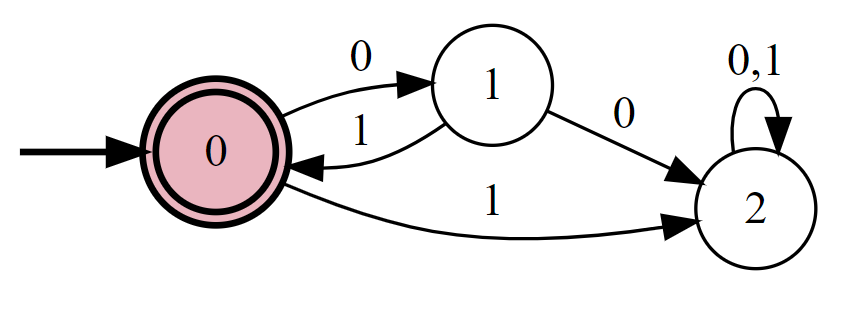
\includegraphics[width=\linewidth, height=1.5in, keepaspectratio]{../figure/automaton.png}
\caption{A deterministic finite automaton that computes the function
\(\Phi_{(01)^*}\).}
\label{automatonregfig}
\end{marginfigure}


\begin{marginfigure}
\centering
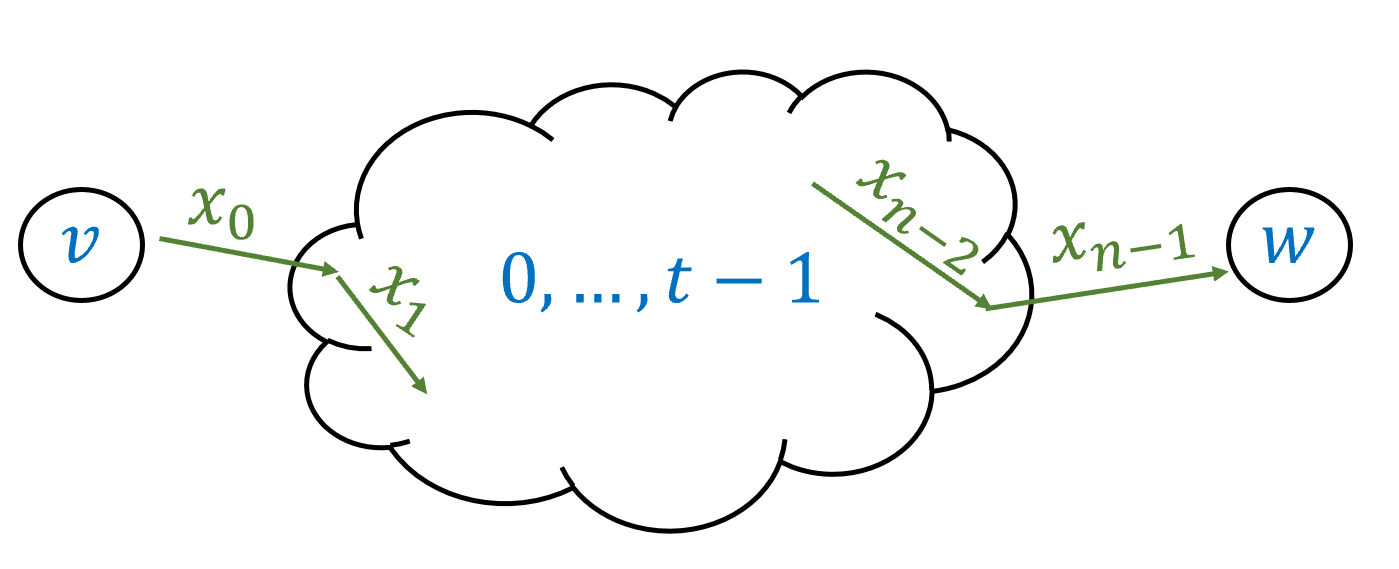
\includegraphics[width=\linewidth, height=1.5in, keepaspectratio]{../figure/dfatoreg1.png}
\caption{Given a DFA of \(C\) states, for every \(v,w \in [C]\) and
number \(t\in \{0,\ldots,C\}\) we define the function
\(F^t_{v,w}:\{0,1\}^* \rightarrow \{0,1\}\) to output one on input
\(x\in \{0,1\}^*\) if and only if when the DFA is initialized in the
state \(v\) and is given the input \(x\), it will teach the state \(w\)
while going only through the intermediate states \(\{0,\ldots,t-1\}\).}
\label{dfatoregonefig}
\end{marginfigure}

\begin{proof}[Proof of \cref{dfaregequivthm}] \label[proof]{Since-crefDFAforREGthm-pr}

Since \cref{DFAforREGthm} proves the ``only if'' direction, we only need
to show the ``if'' direction. Let \(A=(T,\mathcal{S})\) be a DFA with
\(C\) states that computes the function \(F\). We need to show that
\(F\) is regular.

For every \(v,w \in [C]\), we let
\(F_{v,w}:\{0,1\}^* \rightarrow \{0,1\}\) be the function that maps
\(x\in \{0,1\}^*\) to \(1\) if and only if the DFA \(A\), starting at
the state \(v\), will reach the state \(w\) if it reads the input \(x\).
We will prove that \(F_{v,w}\) is regular for every \(v,w\). This will
prove the theorem, since by \cref{DFAdef}, \(F(x)\) is equal to the OR
of \(F_{0,w}(x)\) for every \(w\in \mathcal{S}\). Hence if we have a
regular expression for every function of the form \(F_{v,w}\) then
(using the \(|\) operation) we can obtain a regular expression for \(F\)
as well.

To give regular expressions for the functions \(F_{v,w}\), we start by
defining the following functions \(F_{v,w}^t\): for every
\(v,w \in [C]\) and \(0 \leq t \leq C\), \(F_{v,w}^t(x)=1\) if and only
if starting from \(v\) and observing \(x\), the automata reaches \(w\)
\emph{with all intermediate states being in the set
\([t]=\{0,\ldots, t-1\}\)} (see \cref{dfatoregonefig}). That is, while
\(v,w\) themselves might be outside \([t]\), \(F_{v,w}^t(x)=1\) if and
only if throughout the execution of the automaton on the input \(x\)
(when initiated at \(v\)) it never enters any of the states outside
\([t]\) and still ends up at \(w\). If \(t=0\) then \([t]\) is the empty
set, and hence \(F^0_{v,w}(x)=1\) if and only if the automaton reaches
\(w\) from \(v\) directly on \(x\), without any intermediate state. If
\(t=C\) then all states are in \([t]\), and hence
\(F_{v,w}^t= F_{v,w}\).

We will prove the theorem by induction on \(t\), showing that
\(F^t_{v,w}\) is regular for every \(v,w\) and \(t\). For the
\textbf{base case} of \(t=0\), \(F^0_{v,w}\) is regular for every
\(v,w\) since it can be described as one of the expressions
\(\ensuremath{\text{\texttt{""}}}\), \(\emptyset\), \(0\), \(1\) or
\(0|1\). Specifically, if \(v=w\) then \(F^0_{v,w}(x)=1\) if and only if
\(x\) is the empty string. If \(v\neq w\) then \(F^0_{v,w}(x)=1\) if and
only if \(x\) consists of a single symbol \(\sigma \in \{0,1\}\) and
\(T(v,\sigma)=w\). Therefore in this case \(F^0_{v,w}\) corresponds to
one of the four regular expressions \(0|1\), \(0\), \(1\) or
\(\emptyset\), depending on whether \(A\) transitions to \(w\) from
\(v\) when it reads either \(0\) or \(1\), only one of these symbols, or
neither.

\textbf{Inductive step:} Now that we've seen the base case, let's prove
the general case by induction. Assume, via the induction hypothesis,
that for every \(v',w' \in [C]\), we have a regular expression
\(R_{v,w}^t\) that computes \(F_{v',w'}^t\). We need to prove that
\(F_{v,w}^{t+1}\) is regular for every \(v,w\). If the automaton arrives
from \(v\) to \(w\) using the intermediate states \([t+1]\), then it
visits the \(t\)-th state zero or more times. If the path labeled by
\(x\) causes the automaton to get from \(v\) to \(w\) without visiting
the \(t\)-th state at all, then \(x\) is matched by the regular
expression \(R_{v,w}^t\). If the path labeled by \(x\) causes the
automaton to get from \(v\) to \(w\) while visiting the \(t\)-th state
\(k>0\) times then we can think of this path as:

\begin{itemize}
\item
  First travel from \(v\) to \(t\) using only intermediate states in
  \([t-1]\).
\item
  Then go from \(t\) back to itself \(k-1\) using only intermediate
  states in \([t-1]\)
\item
  Then go from \(t\) to \(w\) using only intermediate states in
  \([t-1]\).
\end{itemize}

Therefore in this case the string \(x\) is matched by the regular
expression \(R_{v,t}^t(R_{t,t}^t)^* R_{t,w}^t\). (See also
\cref{dfatoreginductivefig}.)

Therefore we can compute \(F_{v,w}^{t+1}\) using the regular expression

\[R_{v,w}^t \;|\; R_{v,t}^t(R_{t,t}^t)^* R_{t,w}^t\;.\] This completes
the proof of the inductive step and hence of the theorem.

\end{proof}


\begin{figure}
\centering
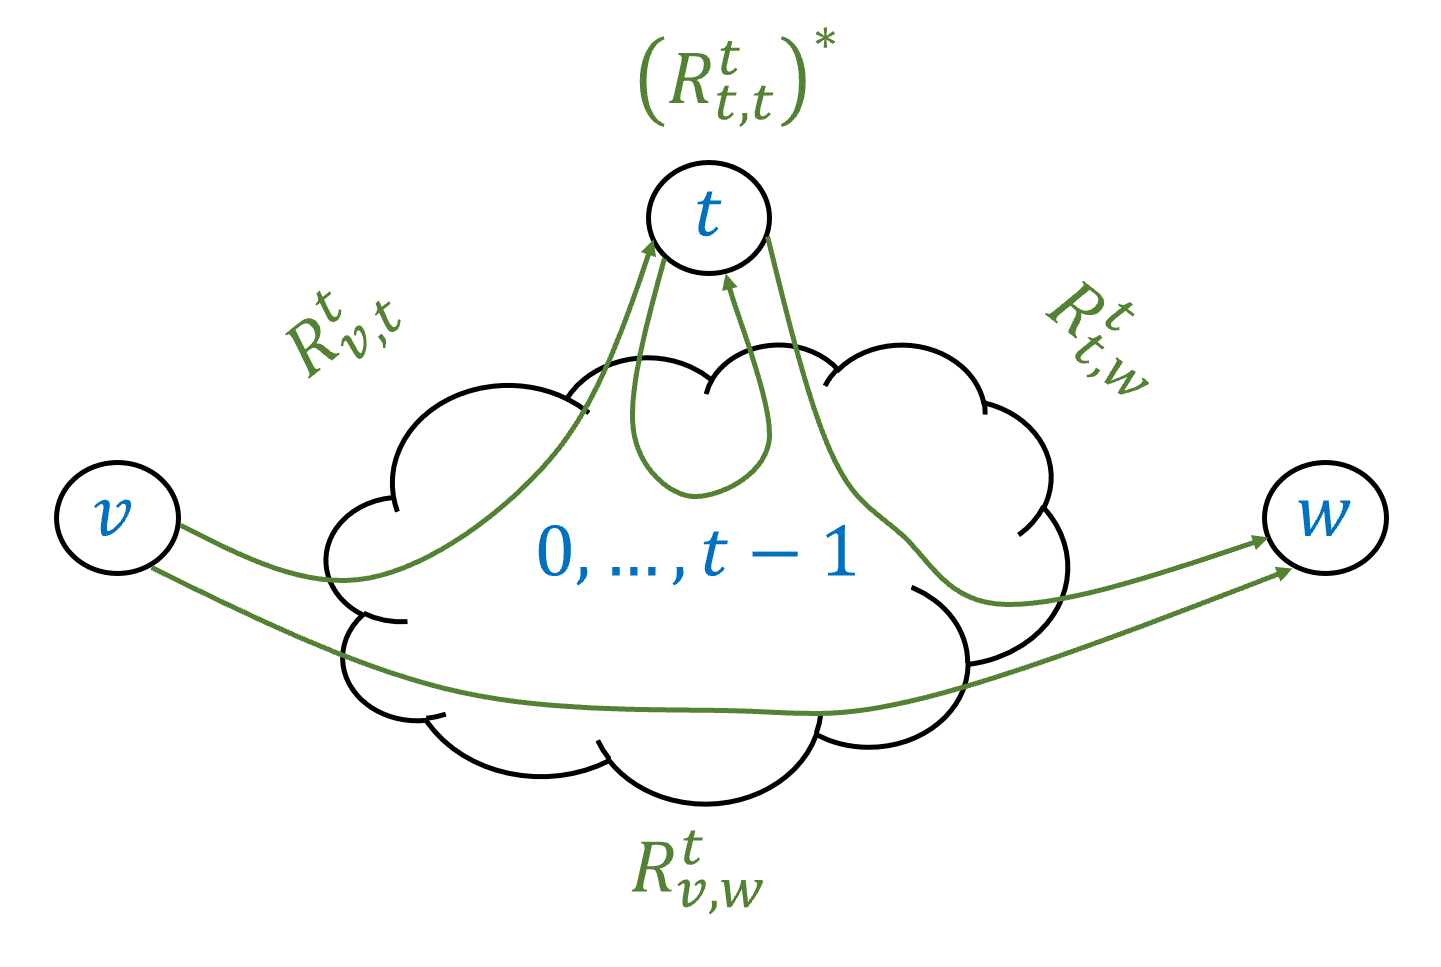
\includegraphics[width=\textwidth, height=0.25\paperheight, keepaspectratio]{../figure/dfatoreginduction.png}
\caption{If we have regular expressions \(R_{v',w'}^{t}\) corresponding
to \(F_{v',w'}^{t}\) for every \(v',w' \in [C]\), we can obtain a
regular expression \(R_{v,w}^{t+1}\) corresponding to \(F_{v,w}^{t+1}\).
The key observation is that a path from \(v\) to \(w\) using
\(\{0,\ldots, t \}\) either does not touch \(t\) at all, in which case
it is captured by the expression \(R_{v,w}^{t}\), or it goes from \(v\)
to \(t\), comes back to \(t\) zero or more times, and then goes from
\(t\) to \(w\), in which case it is captured by the expression
\(R_{v,t}^{t}(R_{t,t}^{t})^* R_{t,w}^t\).}
\label{dfatoreginductivefig}
\end{figure}

\subsection{Regular functions are closed under
complement}\label{Regular-functions-are-clo}

Here is an important corollary of \cref{dfaregequivthm}:

\hypertarget{regcomplementlem}{}
\begin{lemma}[Regular expressions closed under complement] \label[lemma]{regcomplementlem}

If \(F:\{0,1\}^* \rightarrow \{0,1\}\) is regular then so is the
function \(\overline{F}\), where \(\overline{F}(x) = 1 - F(x)\) for
every \(x\in \{0,1\}^*\).

\end{lemma}

\begin{proof} \label[proof]{If-F-is-regular-then-by-c}

If \(F\) is regular then by \cref{reglintimethm} it can be computed by a
constant-space one-pass algorithm \(A\). But then the algorithm
\(\overline{A}\) which does the same computation and outputs the
negation of the output of \(A\) also utilizes constant space and one
pass and computes \(\overline{F}\). By \cref{dfaregequivthm} this
implies that \(\overline{F}\) is regular as well.

\end{proof}

\section{Limitations of regular
expressions}\label{Limitations-of-regular-ex}

The fact that functions computed by regular expressions always halt is
one of the reasons why they are so useful. When you make a regular
expression search, you are guaranteed that that it will terminate with a
result. This is why operating systems and text editors often restrict
their search interface to regular expressions and don't allow searching
by specifying an arbitrary function. But this always-halting property
comes at a cost. Regular expressions cannot compute every function that
is computable by Turing machines. In fact there are some very simple
(and useful!) functions that they cannot compute. Here is one example:

\hypertarget{regexpparn}{}
\begin{lemma}[Matching parenthesis] \label[lemma]{regexpparn}

Let \(\Sigma = \{\langle ,\rangle \}\) and
\(\ensuremath{\mathit{MATCHPAREN}}:\Sigma^* \rightarrow \{0,1\}\) be the
function that given a string of parentheses, outputs \(1\) if and only
if every opening parenthesis is matched by a corresponding closed one.
Then there is no regular expression over \(\Sigma\) that computes
\(\ensuremath{\mathit{MATCHPAREN}}\).

\end{lemma}

\cref{regexpparn} is a consequence of the following result, which is
known as the \emph{pumping lemma}:

\hypertarget{pumping}{}
\begin{theorem}[Pumping Lemma] \label[theorem]{pumping}

Let \(e\) be a regular expression over some alphabet \(\Sigma\). Then
there is some number \(n_0\) such that for every \(w\in \Sigma^*\) with
\(|w|>n_0\) and \(\Phi_{e}(w)=1\), we can write \(w=xyz\) for strings
\(x,y,z \in \Sigma^*\) satisfying the following conditions:

\begin{enumerate}
\def\labelenumi{\arabic{enumi}.}
\item
  \(|y| \geq 1\).
\item
  \(|xy| \leq n_0\).
\item
  \(\Phi_{e}(xy^kz)=1\) for every \(k\in \N\).
\end{enumerate}

\end{theorem}


\begin{figure}
\centering
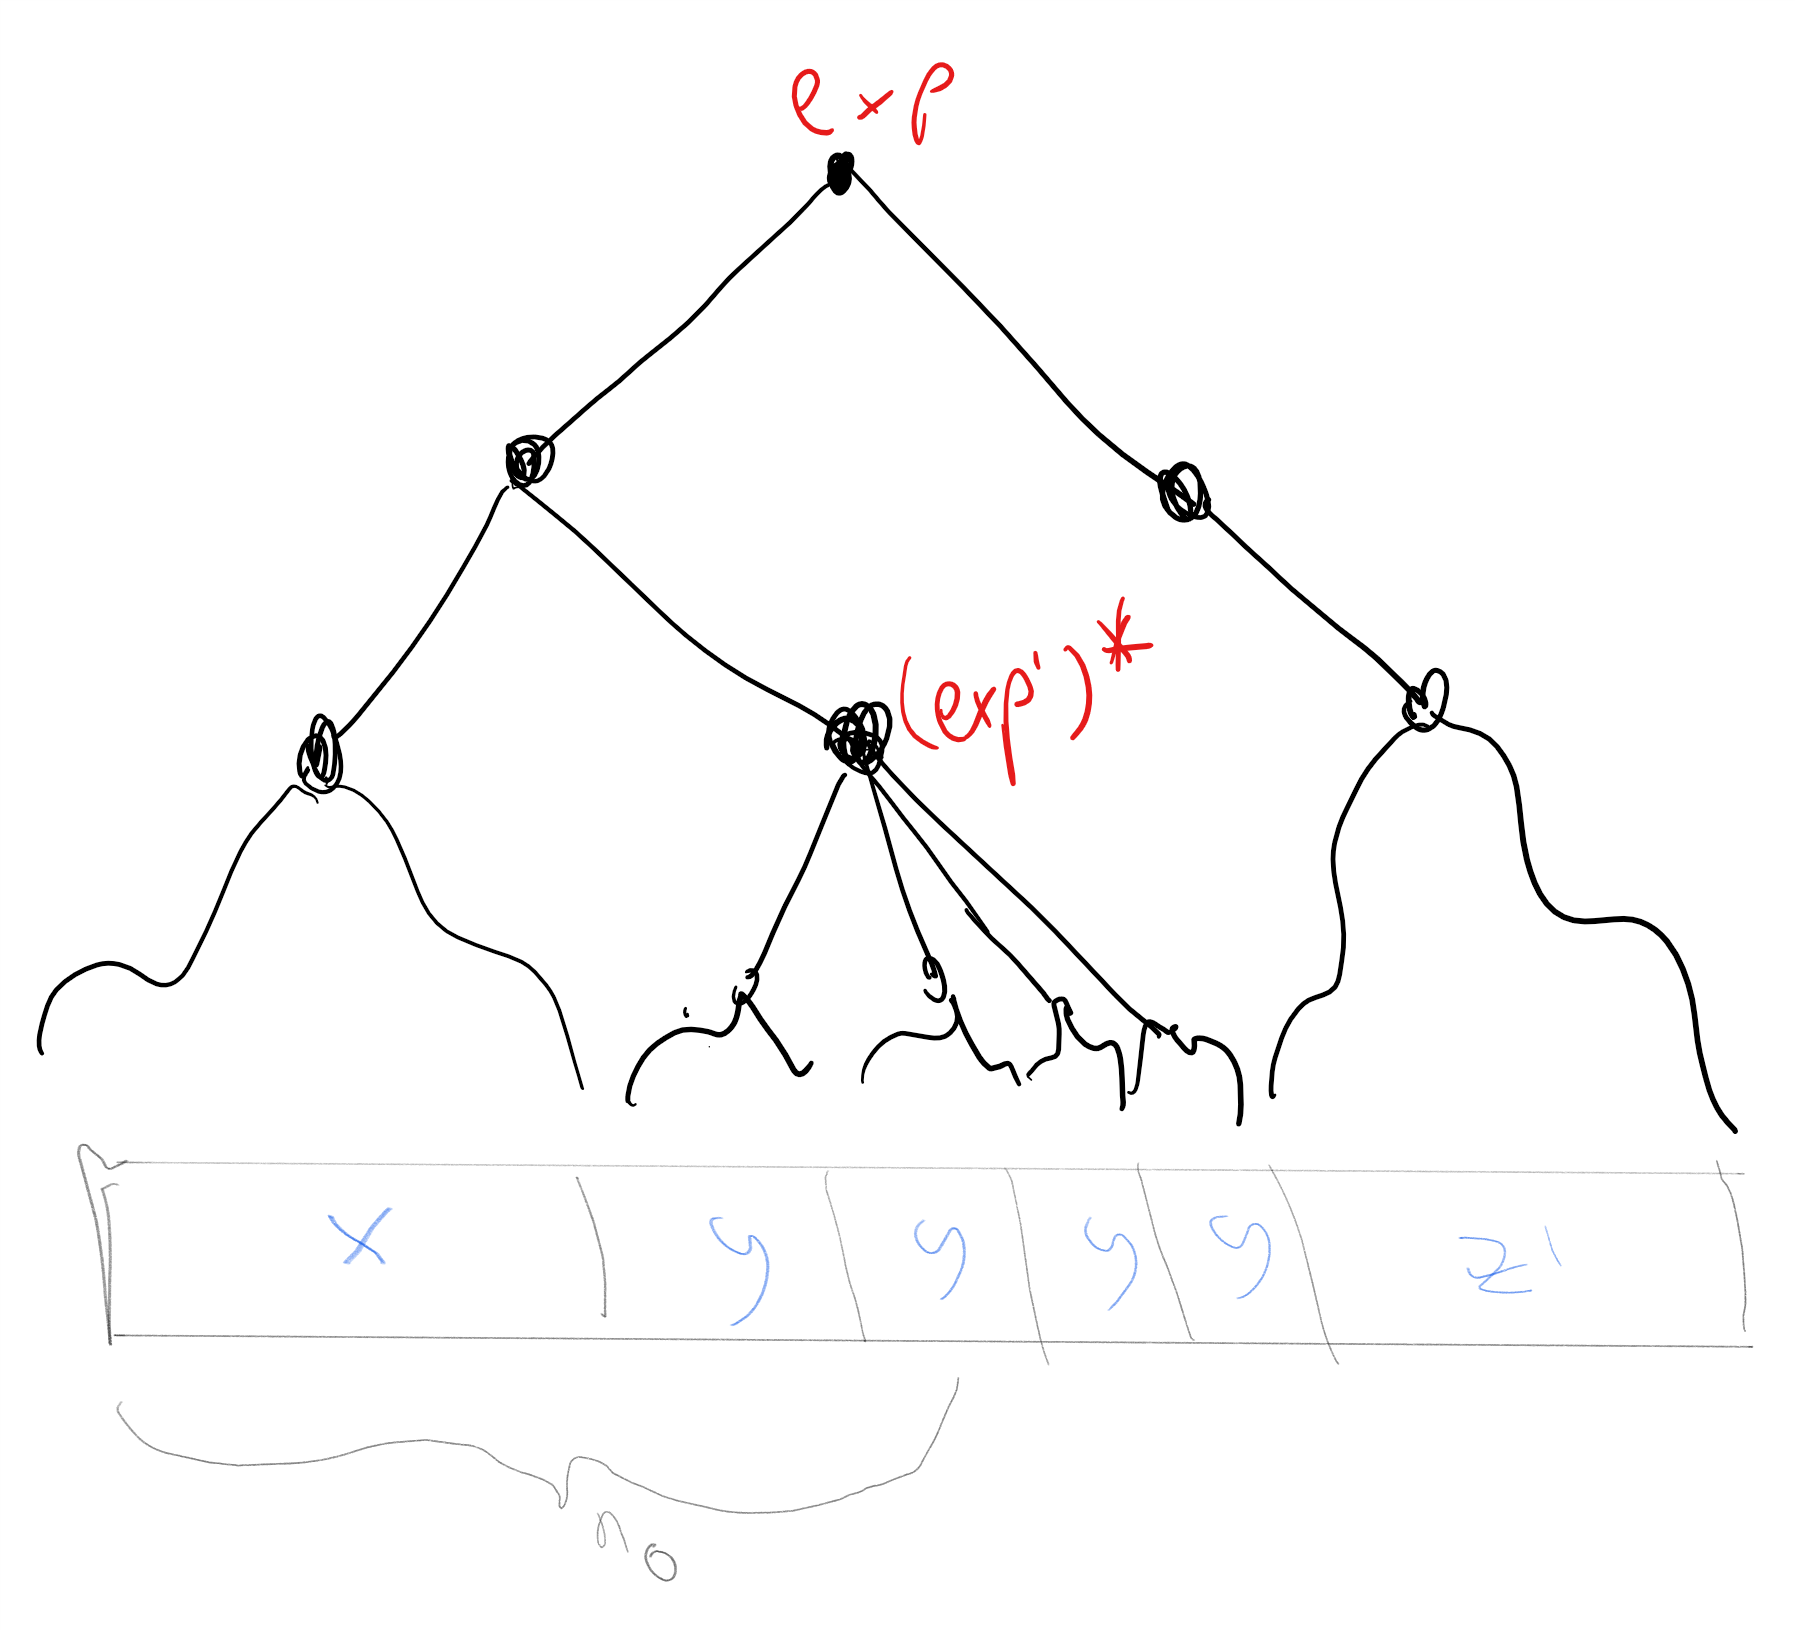
\includegraphics[width=\textwidth, height=0.25\paperheight, keepaspectratio]{../figure/pumpinglemma.png}
\caption{To prove the ``pumping lemma'' we look at a word \(w\) that is
much larger than the regular expression \(e\) that matches it. In such a
case, part of \(w\) must be matched by some sub-expression of the form
\((e')^*\), since this is the only operator that allows matching words
longer than the expression. If we look at the ``leftmost'' such
sub-expression and define \(y^k\) to be the string that is matched by
it, we obtain the partition needed for the pumping lemma.}
\label{pumpinglemmafig}
\end{figure}

\begin{proofidea} \label[proofidea]{The-idea-behind-the-proof}

The idea behind the proof the following. Let \(n_0\) be twice the number
of symbols that are used in the expression \(e\), then the only way that
there is some \(w\) with \(|w|>n_0\) and \(\Phi_{e}(w)=1\) is that \(e\)
contains the \(*\) (i.e.~star) operator and that there is a nonempty
substring \(y\) of \(w\) that was matched by \((e')^*\) for some
sub-expression \(e'\) of \(e\). We can now repeat \(y\) any number of
times and still get a matching string. See also \cref{pumpinglemmafig}.

\end{proofidea}

\begin{pause} \label[pause]{The-pumping-lemma-is-a-bi}

The pumping lemma is a bit cumbersome to state, but one way to remember
it is that it simply says the following: \emph{``if a string matching a
regular expression is long enough, one of its substrings must be matched
using the \(*\) operator''}.

\end{pause}

\begin{proof}[Proof of \cref{pumping}] \label[proof]{To-prove-the-lemma-formal}

To prove the lemma formally, we use induction on the length of the
expression. Like all induction proofs, this is going to be somewhat
lengthy, but at the end of the day it directly follows the intuition
above that \emph{somewhere} we must have used the star operation.
Reading this proof, and in particular understanding how the formal proof
below corresponds to the intuitive idea above, is a very good way to get
more comfortable with inductive proofs of this form.

Our inductive hypothesis is that for an \(n\) length expression,
\(n_0=2n\) satisfies the conditions of the lemma. The \textbf{base case}
is when the expression is a single symbol \(\sigma \in \Sigma\) or that
the expression is \(\emptyset\) or \(\ensuremath{\text{\texttt{""}}}\).
In all these cases the conditions of the lemma are satisfied simply
because there \(n_0=2\) and there is no string \(x\) of length larger
than \(n_0\) that is matched by the expression.

We now prove the \textbf{inductive step}. Let \(e\) be a regular
expression with \(n>1\) symbols. We set \(n_0=2n\) and let
\(w\in \Sigma^*\) be a string satisfying \(|w|>n_0\). Since \(e\) has
more than one symbol, it has one of the the forms \textbf{(a)}
\(e' | e''\), \textbf{(b)}, \((e')(e'')\), or \textbf{(c)} \((e')^*\)
where in all these cases the subexpressions \(e'\) and \(e''\) have
fewer symbols than \(e\) and hence satisfy the induction hypothesis.

In the case \textbf{(a)}, every string \(w\) matched by \(e\) must be
matched by either \(e'\) or \(e''\). If \(e'\) matches \(w\) then, since
\(|w|>2|e'|\), by the induction hypothesis there exist \(x,y,z\) with
\(|y| \geq 1\) and \(|xy| \leq 2|e'| <n_0\) such that \(e'\) (and
therefore also \(e=e'|e''\)) matches \(xy^kz\) for every \(k\). The same
arguments works in the case that \(e''\) matches \(w\).

In the case \textbf{(b)}, if \(w\) is matched by \((e')(e'')\) then we
can write \(w=w'w''\) where \(e'\) matches \(w'\) and \(e''\) matches
\(w''\). We split to subcases. If \(|w'|>2|e'|\) then by the induction
hypothesis there exist \(x,y,z'\) with \(|y| \leq 1\),
\(|xy| \leq 2|e'| < n_0\) such that \(w'=xyz'\) and \(e'\) matches
\(xy^kz'\) for every \(k\in \N\). This completes the proof since if we
set \(z=z'w''\) then we see that \(w=w'w''=xyz\) and \(e=(e')(e'')\)
matches \(xy^kz\) for every \(k\in \N\). Otherwise, if
\(|w'| \leq 2|e'|\) then since \(|w|=|w'|+|w''|>n_0=2(|e'|+|e''|)\), it
must be that \(|w''|>2|e''|\). Hence by the induction hypothesis there
exist \(x',y,z\) such that \(|y| \geq 1\), \(|x'y| \leq 2|e''|\) and
\(e''\) matches \(x'y^kz\) for every \(k\in \N\). But now if we set
\(x=w'x'\) we see that
\(|xy| \leq |w'| + |x'y| \leq 2|e'| + 2|e''| =n_0\) and on the other
hand the expression \(e=(e')(e'')\) matches \(xy^kz = w'x'y^kz\) for
every \(k\in \N\).

In case \textbf{(c)}, if \(w\) is matched \((e')^*\) then
\(w= w_0\cdots w_t\) where for every \(i\in [t]\), \(w_i\) is a nonempty
string matched by \(e'\). If \(|w_0|>2|e'|\) then we can use the same
approach as in the concatenation case above. Otherwise, we simply note
that if \(x\) is the empty string, \(y=w_0\), and \(z=w_1\cdots w_t\)
then \(|xy| \leq n_0\) and \(xy^kz\) is matched by \((e')^*\) for every
\(k\in \N\).

\end{proof}

\hypertarget{recursiveproofs}{}
\begin{remark}[Recursive definitions and inductive proofs] \label[remark]{recursiveproofs}

When an object is \emph{recursively defined} (as in the case of regular
expressions) then it is natural to prove properties of such objects by
\emph{induction}. That is, if we want to prove that all objects of this
type have property \(P\), then it is natural to use an inductive steps
that says that if \(o',o'',o'''\) etc have property \(P\) then so is an
object \(o\) that is obtained by composing them.

\end{remark}

Using the pumping lemma, we can easily prove \cref{regexpparn} (i.e.,
the non-regularity of the ``matching parenthesis'' function):

\begin{proof}[Proof of \cref{regexpparn}] \label[proof]{Suppose-towards-the-sake-}

Suppose, towards the sake of contradiction, that there is an expression
\(e\) such that \(\Phi_{e}= \ensuremath{\mathit{MATCHPAREN}}\). Let
\(n_0\) be the number obtained from \cref{pumping} and let
\(w =\langle^{n_0}\rangle^{n_0}\) (i.e., \(n_0\) left parenthesis
followed by \(n_0\) right parenthesis). Then we see that if we write
\(w=xyz\) as in \cref{regexpparn}, the condition \(|xy| \leq n_0\)
implies that \(y\) consists solely of left parenthesis. Hence the string
\(xy^2z\) will contain more left parenthesis than right parenthesis.
Hence \(\ensuremath{\mathit{MATCHPAREN}}(xy^2z)=0\) but by the pumping
lemma \(\Phi_{e}(xy^2z)=1\), contradicting our assumption that
\(\Phi_{e}=\ensuremath{\mathit{MATCHPAREN}}\).

\end{proof}

The pumping lemma is a very useful tool to show that certain functions
are \emph{not} computable by a regular expression. However, it is
\emph{not} an ``if and only if'' condition for regularity: there are non
regular functions that still satisfy the conditions of the pumping
lemma. To understand the pumping lemma, it is important to follow the
order of quantifiers in \cref{pumping}. In particular, the number
\(n_0\) in the statement of \cref{pumping} depends on the regular
expression (in the proof we chose \(n_0\) to be twice the number of
symbols in the expression). So, if we want to use the pumping lemma to
rule out the existence of a regular expression \(e\) computing some
function \(F\), we need to be able to choose an appropriate input
\(w\in \{0,1\}^*\) that can be arbitrarily large and satisfies
\(F(w)=1\). This makes sense if you think about the intuition behind the
pumping lemma: we need \(w\) to be large enough as to force the use of
the star operator.


\begin{figure*}

\classiccaptionstyle\centering
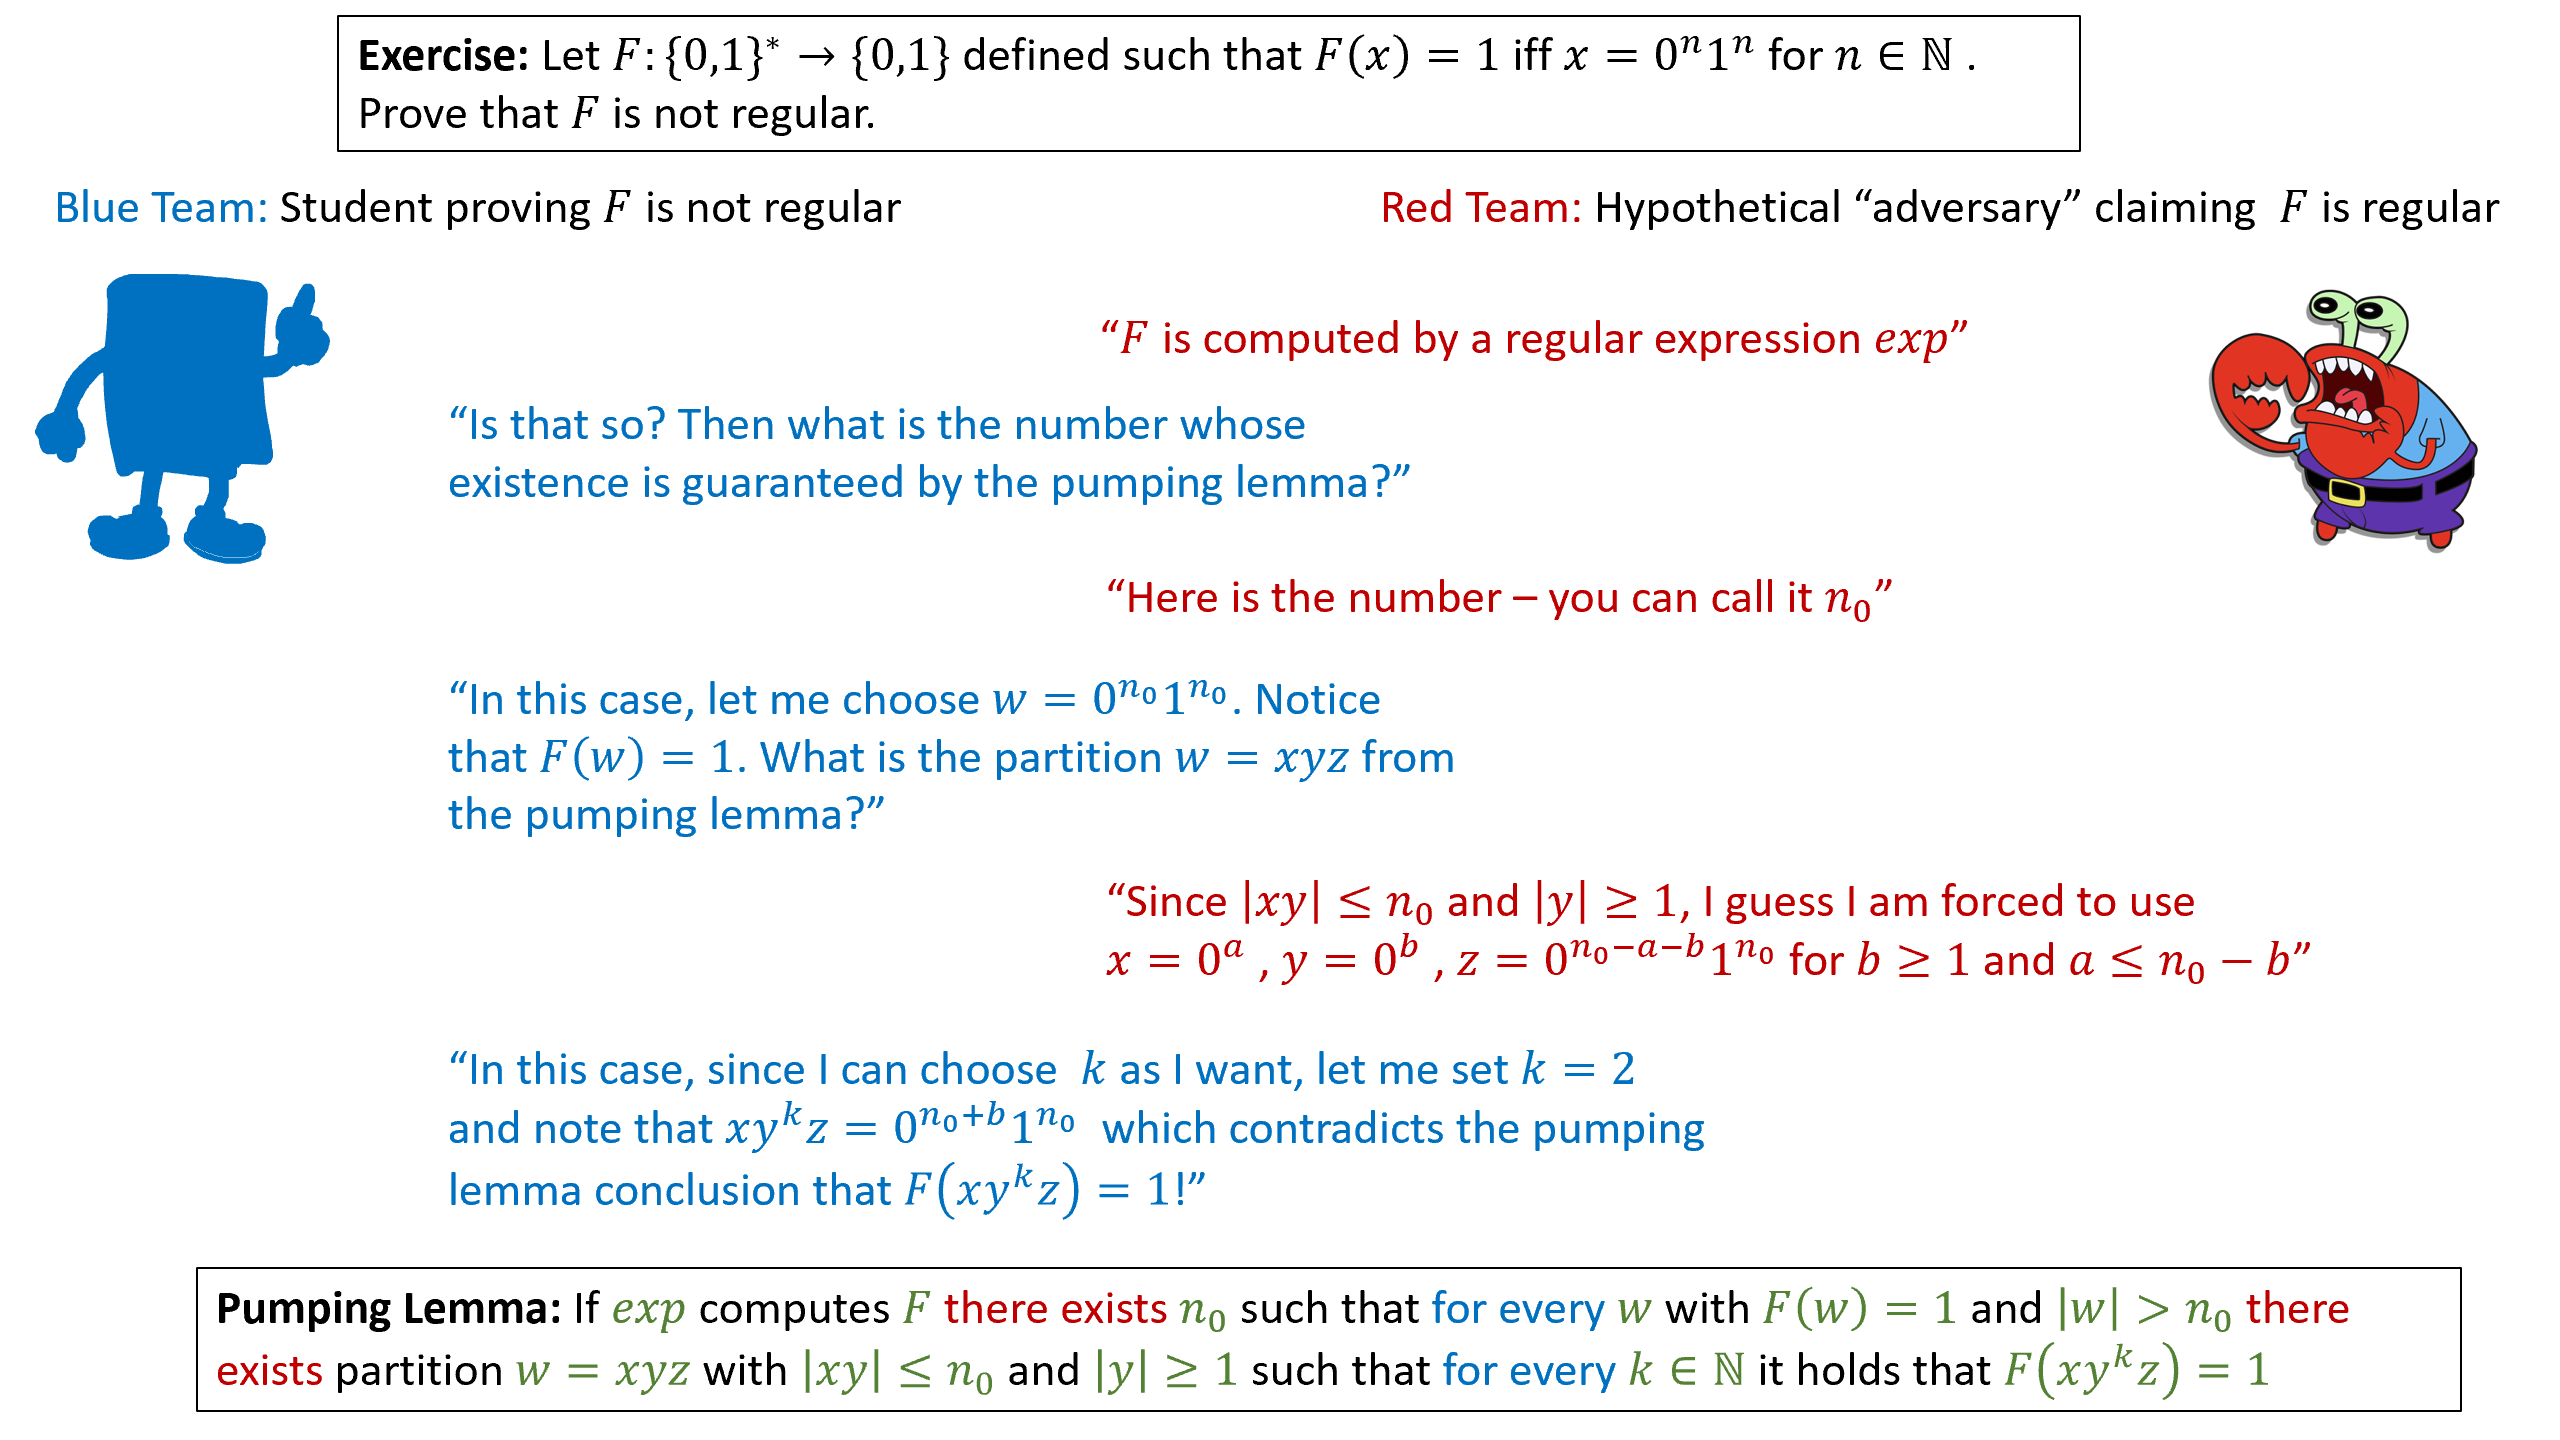
\includegraphics[width=0.9\paperwidth, height=0.3\paperheight, keepaspectratio]{../figure/pumpinglemmaproof.png}
\caption{A cartoon of a proof using the pumping lemma that a function
\(F\) is not regular. The pumping lemma states that if \(F\) is regular
then \emph{there exists} a number \(n_0\) such that \emph{for every}
large enough \(w\) with \(F(w)=1\), \emph{there exists} a partition of
\(w\) to \(w=xyz\) satisfying certain conditions such that \emph{for
every} \(k\in \N\), \(F(xy^kz)=1\). You can imagine a pumping-lemma
based proof as a game between you and the adversary. Every \emph{there
exists} quantifier corresponds to an object you are free to choose on
your own (and base your choice on previously chosen objects). Every
\emph{for every} quantifier corresponds to an object the adversary can
choose arbitrarily (and again based on prior choices) as long as it
satisfies the conditions. A valid proof corresponds to a strategy by
which no matter what the adversary does, you can win the game by
obtaining a contradiction which would be a choice of \(k\) that would
result in \(F(xy^ky)=0\), hence violating the conclusion of the pumping
lemma.}
\label{pumpingprooffig}
\end{figure*}

\hypertarget{palindromenotreg}{}
\begin{solvedexercise}[Palindromes is not regular] \label[solvedexercise]{palindromenotreg}

Prove that the following function over the alphabet \(\{0,1,; \}\) is
not regular: \(\ensuremath{\mathit{PAL}}(w)=1\) if and only if
\(w = u;u^R\) where \(u \in \{0,1\}^*\) and \(u^R\) denotes \(u\)
``reversed'': the string \(u_{|u|-1}\cdots u_0\). (The \emph{Palindrome}
function is most often defined without an explicit separator character
\(;\), but the version with such a separator is a bit cleaner and so we
use it here. This does not make much difference, as one can easily
encode the separator as a special binary string instead.)

\end{solvedexercise}

\begin{solution} \label[solution]{We-use-the-pumping-lemma-}

We use the pumping lemma. Suppose towards the sake of contradiction that
there is a regular expression \(e\) computing
\(\ensuremath{\mathit{PAL}}\), and let \(n_0\) be the number obtained by
the pumping lemma (\cref{pumping}). Consider the string
\(w = 0^{n_0};0^{n_0}\). Since the reverse of the all zero string is the
all zero string, \(\ensuremath{\mathit{PAL}}(w)=1\). Now, by the pumping
lemma, if \(\ensuremath{\mathit{PAL}}\) is computed by \(e\), then we
can write \(w=xyz\) such that \(|xy| \leq n_0\), \(|y|\geq 1\) and
\(\ensuremath{\mathit{PAL}}(xy^kz)=1\) for every \(k\in \N\). In
particular, it must hold that \(\ensuremath{\mathit{PAL}}(xz)=1\), but
this is a contradiction, since \(xz=0^{n_0-|y|};0^{n_0}\) and so its two
parts are not of the same length and in particular are not the reverse
of one another.

\end{solution}

For yet another example of a pumping-lemma based proof, see
\cref{pumpingprooffig} which illustrates a cartoon of the proof of the
non-regularity of the function \(F:\{0,1\}^* \rightarrow \{0,1\}\) which
is defined as \(F(x)=1\) iff \(x=0^n1^n\) for some \(n\in \N\) (i.e.,
\(x\) consists of a string of consecutive zeroes, followed by a string
of consecutive ones of the same length).

\section{Other semantic properties of regular
expressions}\label{Other-semantic-properties}

Regular expressions are widely used beyond just searching. For example,
regular expressions are often used to define \emph{tokens} (such as what
is a valid variable identifier, or keyword) in programming languages.
But they also have other uses. One nice example is the recent work on
the \href{https://goo.gl/oeJNuw}{NetKAT network programming language}.
In recent years, the world of networking moved from fixed topologies to
``software defined networks''. These are run by programmable switches
that can implement policies such as ``if packet is secured by SSL then
forward it to A, otherwise forward it to B''. By its nature, one would
want to use a formalism for such policies that is guaranteed to always
halt (and quickly!) and such that it is possible to answer semantic
questions such as ``does C see the packets moved from A to B'' etc. The
NetKAT language uses a variant of regular expressions to achieve
precisely that.

Such applications use the fact that because regular expressions are so
restricted, we can not only solve the halting problem for them, but also
answer other \emph{semantic questions}. Such semantic questions would
not be solvable for Turing-complete models due to Rice's Theorem
(\cref{rice-thm}). For example, we can tell whether two regular
expressions are \emph{equivalent}, as well as whether a regular
expression computes the constant zero function.

\hypertarget{regemptynessthm}{}
\begin{theorem}[Emptiness of regular languages is computable] \label[theorem]{regemptynessthm}

There is an algorithm that given a regular expression \(e\), outputs
\(1\) if and only if \(\Phi_{e}\) is the constant zero function.

\end{theorem}

\begin{proofidea} \label[proofidea]{The-idea-is-that-we-can-d}

The idea is that we can directly observe this from the structure of the
expression. The only way a regular expression \(e\) computes the
constant zero function is if \(e\) has the form \(\emptyset\) or is
obtained by concatenating \(\emptyset\) with other expressions.

\end{proofidea}

\begin{proof}[Proof of \cref{regemptynessthm}] \label[proof]{Define-a-regular-expressi}

Define a regular expression to be ``empty'' if it computes the constant
zero function. Given a regular expression \(e\), we can determine if
\(e\) is empty using the following rules:

\begin{itemize}
\item
  If \(e\) has the form \(\sigma\) or
  \(\ensuremath{\text{\texttt{""}}}\) then it is not empty.
\item
  If \(e\) is not empty then \(e|e'\) is not empty for every \(e'\).
\item
  If \(e\) is not empty then \(e^*\) is not empty.
\item
  If \(e\) and \(e'\) are both not empty then \(e\; e'\) is not empty.
\item
  \(\emptyset\) is empty.
\end{itemize}

Using these rules it is straightforward to come up with a recursive
algorithm to determine emptiness.

\end{proof}

\hypertarget{regequivalencethm}{}
\begin{theorem}[Equivalence of regular expressions is computable] \label[theorem]{regequivalencethm}

Let \(\ensuremath{\mathit{REGEQ}}:\{0,1\}^* \rightarrow \{0,1\}\) be the
function that on input (a string representing) a pair of regular
expressions \(e,e'\), \(\ensuremath{\mathit{REGEQ}}(e,e')=1\) if and
only if \(\Phi_{e} = \Phi_{e'}\). Then \(\ensuremath{\mathit{REGEQ}}\)
is computable.

\end{theorem}

\begin{proofidea} \label[proofidea]{The-idea-is-to-show-that-}

The idea is to show that given a pair of regular expression \(e\) and
\(e'\) we can find an expression \(e''\) such that \(\Phi_{e''}(x)=1\)
if and only if \(\Phi_e(x) \neq \Phi_(e'')(x)\). Therefore
\(\Phi_{e''}\) is the constant zero function if and only if \(e\) and
\(e'\) are equivalent, and thus we can test for emptiness of \(e''\) to
determine equivalence of \(e\) and \(e'\).

\end{proofidea}

\begin{proof}[Proof of \cref{regequivalencethm}] \label[proof]{We-will-prove-crefregequi}

We will prove \cref{regequivalencethm} from \cref{regemptynessthm}. (The
two theorems are in fact equivalent: it is easy to prove
\cref{regemptynessthm} from \cref{regequivalencethm}, since checking for
emptiness is the same as checking equivalence with the expression
\(\emptyset\).) Given two regular expressions \(e\) and \(e'\), we will
compute an expression \(e''\) such that \(\Phi_{e''}(x) =1\) if and only
if \(\Phi_e(x) \neq \Phi_{e'}(x)\). One can see that \(e\) is equivalent
to \(e'\) if and only if \(e''\) is empty.

We start with the observation that for every bit \(a,b \in \{0,1\}\),
\(a \neq b\) if and only if \[
(a \wedge \overline{b}) \; \vee \;  (\overline{a} \wedge b) \;.
\]

Hence we need to construct \(e''\) such that for every \(x\),

\[
\Phi_{e''}(x) = (\Phi_{e}(x) \wedge \overline{\Phi_{e'}(x)}) \; \vee  \; (\overline{\Phi_{e}(x)} \wedge \Phi_{e'}(x)) \;.
\label{eqemptyequivreg}
\]

To construct the expression \(e''\), we will show how given any pair of
expressions \(e\) and \(e'\), we can construct expressions
\(e\wedge e'\) and \(\overline{e}\) that compute the functions
\(\Phi_{e} \wedge \Phi_{e'}\) and \(\overline{\Phi_{e}}\) respectively.
(Computing the expression for \(e \vee e'\) is straightforward using the
\(|\) operation of regular expressions.)

Specifically, by \cref{regcomplementlem}, regular functions are closed
under negation, which means that for every regular expression \(e\),
there is an expression \(\overline{e}\) such that
\(\Phi_{\overline{e}}(x) = 1 - \Phi_{e}(x)\) for every
\(x\in \{0,1\}^*\). Now, for every two expression \(e\) and \(e'\), the
expression \[
e \wedge e' = \overline{(\overline{e} | \overline{e'})}
\] computes the AND of the two expressions. Given these two
transformations, we see that for every regular expressions \(e\) and
\(e'\) we can find a regular expression \(e''\) satisfying
\eqref{eqemptyequivreg} such that \(e''\) is empty if and only if \(e\)
and \(e'\) are equivalent.

\end{proof}

\section{Context free grammars}\label{seccfg}

If you have ever written a program, you've experienced a \emph{syntax
error}. You probably also had the experience of your program entering
into an \emph{infinite loop}. What is less likely is that the compiler
or interpreter entered an infinite loop while trying to figure out if
your program has a syntax error.

When a person designs a programming language, they need to determine its
\emph{syntax}. That is, the designer decides which strings corresponds
to valid programs, and which ones do not (i.e., which strings contain a
syntax error). To ensure that a compiler or interpreter always halts
when checking for syntax errors, language designers typically \emph{do
not} use a general Turing-complete mechanism to express their syntax.
Rather they use a \emph{restricted} computational model. One of the most
popular choices for such models is \emph{context free grammars}.

To explain context free grammars, let us begin with a canonical example.
Consider the function
\(\ensuremath{\mathit{ARITH}}:\Sigma^* \rightarrow \{0,1\}\) that takes
as input a string \(x\) over the alphabet
\(\Sigma = \{ (,),+,-,\times,\div,0,1,2,3,4,5,6,7,8,9\}\) and returns
\(1\) if and only if the string \(x\) represents a valid arithmetic
expression. Intuitively, we build expressions by applying an operation
such as \(+\),\(-\),\(\times\) or \(\div\) to smaller expressions, or
enclosing them in parenthesis, where the ``base case'' corresponds to
expressions that are simply numbers. More precisely, we can make the
following definitions:

\begin{itemize}
\item
  A \emph{digit} is one of the symbols \(0,1,2,3,4,5,6,7,8,9\).
\item
  A \emph{number} is a sequence of digits. (For simplicity we drop the
  condition that the sequence does not have a leading zero, though it is
  not hard to encode it in a context-free grammar as well.)
\item
  An \emph{operation} is one of \(+,-,\times,\div\)
\item
  An \emph{expression} has either the form ``\emph{number}'', the form
  ``\emph{sub-expression1 operation sub-expression2}'', or the form
  ``(\emph{sub-expression1})'', where ``sub-expression1'' and
  ``sub-expression2'' are themselves expressions. (Note that this is a
  \emph{recursive} definition.)
\end{itemize}

A context free grammar (CFG) is a formal way of specifying such
conditions. A CFG consists of a set of \emph{rules} that tell us how to
generate strings from smaller components. In the above example, one of
the rules is ``if \(exp1\) and \(exp2\) are valid expressions, then
\(exp1 \times exp2\) is also a valid expression''; we can also write
this rule using the shorthand
\(expression \; \Rightarrow \; expression \; \times \; expression\). As
in the above example, the rules of a context-free grammar are often
\emph{recursive}: the rule
\(expression \; \Rightarrow\; expression \; \times \; expression\)
defines valid expressions in terms of itself. We now formally define
context-free grammars:

\hypertarget{defcfg}{}
\begin{definition}[Context Free Grammar] \label[definition]{defcfg}

Let \(\Sigma\) be some finite set. A \emph{context free grammar (CFG)
over \(\Sigma\)} is a triple \((V,R,s)\) such that:

\begin{itemize}
\item
  \(V\), known as the \emph{variables}, is a set disjoint from
  \(\Sigma\).
\item
  \(v\in V\) is known as the \emph{initial variable}.
\item
  \(R\) is a set of \emph{rules}. Each rule is a pair \((v,z)\) with
  \(v\in V\) and \(z\in (\Sigma \cup V)^*\). We often write the rule
  \((v,z)\) as \(v \Rightarrow z\) and say that the string \(z\)
  \emph{can be derived} from the variable \(v\).
\end{itemize}

\end{definition}

\hypertarget{cfgarithmeticex}{}
\begin{example}[Context free grammar for arithmetic expressions] \label[example]{cfgarithmeticex}

The example above of well-formed arithmetic expressions can be captured
formally by the following context free grammar:

\begin{itemize}
\item
  The alphabet \(\Sigma\) is
  \(\{ (,),+,-,\times,\div,0,1,2,3,4,5,6,7,8,9\}\)
\item
  The variables are
  \(V = \{ expression \;,\; number \;,\; digit \;,\; operation \}\).
\item
  The rules are the set \(R\) containing the following \(19\) rules:

  \begin{itemize}
  \item
    The \(4\) rules \(operation \Rightarrow +\),
    \(operation \Rightarrow -\), \(operation \Rightarrow \times\), and
    \(operation \Rightarrow \div\).
  \item
    The \(10\) rules \(digit \Rightarrow 0\),\(\ldots\),
    \(digit \Rightarrow 9\).
  \item
    The rule \(number \Rightarrow digit\).
  \item
    The rule \(number \Rightarrow digit\; number\).
  \item
    The rule \(expression \Rightarrow number\).
  \item
    The rule
    \(expression \Rightarrow expression \; operation \; expression\).
  \item
    The rule \(expression \Rightarrow (expression)\).
  \end{itemize}
\item
  The starting variable is \(expression\)
\end{itemize}

\end{example}

People use many different notations to write context free grammars. One
of the most common notations is the
\href{https://goo.gl/R4qZji}{Backus--Naur form}. In this notation we
write a rule of the form \(v \Rightarrow a\) (where \(v\) is a variable
and \(a\) is a string) in the form \texttt{<v> := a}. If we have several
rules of the form \(v \mapsto a\), \(v \mapsto b\), and \(v \mapsto c\)
then we can combine them as \texttt{<v> := a|b|c}. (In words we say that
\(v\) can derive either \(a\), \(b\), or \(c\).) For example, the
Backus-Naur description for the context free grammar of
\cref{cfgarithmeticex} is the following (using ASCII equivalents for
operations):

\begin{code}
operation  := +|-|*|/
digit      := 0|1|2|3|4|5|6|7|8|9
number     := digit|digit number
expression := number|expression operation expression|(expression)
\end{code}

Another example of a context free grammar is the ``matching
parenthesis'' grammar, which can be represented in Backus-Naur as
follows:

\begin{code}
match  := ""|match match|(match)
\end{code}

A string over the alphabet \(\{\) \texttt{(},\texttt{)} \(\}\) can be
generated from this grammar (where \texttt{match} is the starting
expression and \texttt{""} corresponds to the empty string) if and only
if it consists of a matching set of parenthesis. In contrast, by
\cref{regexpparn} there is no regular expression that matches a string
\(x\) if and only if \(x\) contains a valid sequence of matching
parenthesis.

\subsection{Context-free grammars as a computational
model}\label{Context-free-grammars-as-}

We can think of a context-free grammar over the alphabet \(\Sigma\) as
defining a function that maps every string \(x\) in \(\Sigma^*\) to
\(1\) or \(0\) depending on whether \(x\) can be generated by the rules
of the grammars. We now make this definition formally.

\hypertarget{CFGderive}{}
\begin{definition}[Deriving a string from a grammar] \label[definition]{CFGderive}

If \(G=(V,R,s)\) is a context-free grammar over \(\Sigma\), then for two
strings \(\alpha,\beta \in (\Sigma \cup V)^*\) we say that \(\beta\)
\emph{can be derived in one step} from \(\alpha\), denoted by
\(\alpha \Rightarrow_G \beta\), if we can obtain \(\beta\) from
\(\alpha\) by applying one of the rules of \(G\). That is, we obtain
\(\beta\) by replacing in \(\alpha\) one occurrence of the variable
\(v\) with the string \(z\), where \(v \Rightarrow z\) is a rule of
\(G\).

We say that \(\beta\) \emph{can be derived} from \(\alpha\), denoted by
\(\alpha \Rightarrow_G^* \beta\), if it can be derived by some finite
number \(k\) of steps. That is, if there are
\(\alpha_1,\ldots,\alpha_{k-1} \in (\Sigma \cup V)^*\), so that
\(\alpha \Rightarrow_G \alpha_1 \Rightarrow_G \alpha_2 \Rightarrow_G \cdots \Rightarrow_G \alpha_{k-1} \Rightarrow_G \beta\).

We say that \(x\in \Sigma^*\) is \emph{matched} by \(G=(V,R,s)\) if
\(x\) can be derived from the starting variable \(s\) (i.e., if
\(s \Rightarrow_G^* x\)). We define the \emph{function computed by}
\((V,R,s)\) to be the map \(\Phi_{V,R,s}:\Sigma^* \rightarrow \{0,1\}\)
such that \(\Phi_{V,R,s}(x)=1\) iff \(x\) is matched by \((V,R,s)\). A
function \(F:\Sigma^* \rightarrow \{0,1\}\) is \emph{context free} if
\(F = \Phi_{V,R,s}\) for some CFG \((V,R,s)\).\footnote{As in the case
  of \cref{matchingregexpdef} we can also use \emph{language} rather
  than \emph{function} notation and say that a language
  \(L \subseteq \Sigma^*\) is \emph{context free} if the function \(F\)
  such that \(F(x)=1\) iff \(x\in L\) is context free.}

\end{definition}

A priori it might not be clear that the map \(\Phi_{V,R,s}\) is
computable, but it turns out that this is the case.

\hypertarget{CFGhalt}{}
\begin{theorem}[Context-free grammars always halt] \label[theorem]{CFGhalt}

For every CFG \((V,R,s)\) over \(\{0,1\}\), the function
\(\Phi_{V,R,s}:\{0,1\}^* \rightarrow \{0,1\}\) is computable.

\end{theorem}

As usual we restrict attention to grammars over \(\{0,1\}\) although the
proof extends to any finite alphabet \(\Sigma\).

\begin{proof} \label[proof]{We-only-sketch-the-proof-}

We only sketch the proof. We start with the observation we can convert
every CFG to an equivalent version of \emph{Chomsky normal form}, where
all rules either have the form \(u \rightarrow vw\) for variables
\(u,v,w\) or the form \(u \rightarrow \sigma\) for a variable \(u\) and
symbol \(\sigma \in \Sigma\), plus potentially the rule
\(s \rightarrow \ensuremath{\text{\texttt{""}}}\) where \(s\) is the
starting variable.

The idea behind such a transformation is to simply add new variables as
needed, and so for example we can translate a rule such as
\(v \rightarrow u\sigma w\) into the three rules \(v \rightarrow ur\),
\(r \rightarrow tw\) and \(t \rightarrow \sigma\).

Using the Chomsky Normal form we get a natural recursive algorithm for
computing whether \(s \Rightarrow_G^* x\) for a given grammar \(G\) and
string \(x\). We simply try all possible guesses for the first rule
\(s \rightarrow uv\) that is used in such a derivation, and then all
possible ways to partition \(x\) as a concatenation \(x=x'x''\). If we
guessed the rule and the partition correctly, then this reduces our task
to checking whether \(u \Rightarrow_G^* x'\) and
\(v \Rightarrow_G^* x''\), which (as it involves shorter strings) can be
done recursively. The base cases are when \(x\) is empty or a single
symbol, and can be easily handled.

\end{proof}

\hypertarget{parsetreesrem}{}
\begin{remark}[Parse trees] \label[remark]{parsetreesrem}

While we focus on the task of \emph{deciding} whether a CFG matches a
string, the algorithm to compute \(\Phi_{V,R,s}\) actually gives more
information than that. That is, on input a string \(x\), if
\(\Phi_{V,R,s}(x)=1\) then the algorithm yields the sequence of rules
that one can apply from the starting vertex \(s\) to obtain the final
string \(x\). We can think of these rules as determining a \emph{tree}
with \(s\) being the \emph{root} vertex and the sinks (or \emph{leaves})
corresponding to the substrings of \(x\) that are obtained by the rules
that do not have a variable in their second element. This tree is known
as the \emph{parse tree} of \(x\), and often yields very useful
information about the structure of \(x\).

Often the first step in a compiler or interpreter for a programming
language is a \emph{parser} that transforms the source into the parse
tree (also known as the
\href{https://en.wikipedia.org/wiki/Abstract_syntax_tree}{abstract
syntax tree}). There are also tools that can automatically convert a
description of a context-free grammars into a parser algorithm that
computes the parse tree of a given string. (Indeed, the above recursive
algorithm can be used to achieve this, but there are much more efficient
versions, especially for grammars that have
\href{https://en.wikipedia.org/wiki/LR_parser}{particular forms}, and
programming language designers often try to ensure their languages have
these more efficient grammars.)

\end{remark}

\subsection{The power of context free
grammars}\label{The-power-of-context-free}

Context free grammars can capture every regular expression:

\hypertarget{CFGreg}{}
\begin{theorem}[Context free grammars and regular expressions] \label[theorem]{CFGreg}

Let \(e\) be a regular expression over \(\{0,1\}\), then there is a CFG
\((V,R,s)\) over \(\{0,1\}\) such that \(\Phi_{V,R,s}=\Phi_{e}\).

\end{theorem}

\begin{proof} \label[proof]{We-prove-the-theorem-by-i}

We prove the theorem by induction on the length of \(e\). If \(e\) is an
expression of one bit length, then \(e=0\) or \(e=1\), in which case we
leave it to the reader to verify that there is a (trivial) CFG that
computes it. Otherwise, we fall into one of the following case:
\textbf{case 1:} \(e = e'e''\), \textbf{case 2:} \(e = e'|e''\) or
\textbf{case 3:} \(e=(e')^*\) where in all cases \(e',e''\) are shorter
regular expressions. By the induction hypothesis have grammars
\((V',R',s')\) and \((V'',R'',s'')\) that compute \(\Phi_{e'}\) and
\(\Phi_{e''}\) respectively. By renaming of variables, we can also
assume without loss of generality that \(V'\) and \(V''\) are disjoint.

In case 1, we can define the new grammar as follows: we add a new
starting variable \(s \not\in V \cup V'\) and the rule
\(s \mapsto s's''\). In case 2, we can define the new grammar as
follows: we add a new starting variable \(s \not\in V \cup V'\) and the
rules \(s \mapsto s'\) and \(s \mapsto s''\). Case 3 will be the only
one that uses \emph{recursion}. As before we add a new starting variable
\(s \not\in V \cup V'\), but now add the rules
\(s \mapsto \ensuremath{\text{\texttt{""}}}\) (i.e., the empty string)
and also add, for every rule of the form \((s',\alpha) \in R'\), the
rule \(s \mapsto s\alpha\) to \(R\).

We leave it to the reader as (a very good!) exercise to verify that in
all three cases the grammars we produce capture the same function as the
original expression.

\end{proof}

It turns out that CFG's are strictly more powerful than regular
expressions. In particular, as we've seen, the ``matching parenthesis''
function \(\ensuremath{\mathit{MATCHPAREN}}\) can be computed by a
context free grammar, whereas, as shown in \cref{regexpparn}, it cannot
be computed by regular expressions. Here is another example:

\hypertarget{reversedstringcfg}{}
\begin{solvedexercise}[Context free grammar for palindromes] \label[solvedexercise]{reversedstringcfg}

Let \(\ensuremath{\mathit{PAL}}:\{0,1,;\}^* \rightarrow \{0,1\}\) be the
function defined in \cref{palindromenotreg} where
\(\ensuremath{\mathit{PAL}}(w)=1\) iff \(w\) has the form \(u;u^R\).
Then \(\ensuremath{\mathit{PAL}}\) can be computed by a context-free
grammar

\end{solvedexercise}

\begin{solution} \label[solution]{A-simple-grammar-computin}

A simple grammar computing \(\ensuremath{\mathit{PAL}}\) can be
described using Backus--Naur notation:

\begin{code}
start      := ; | 0 start 0 | 1 start 1
\end{code}

One can prove by induction that this grammar generates exactly the
strings \(w\) such that \(\ensuremath{\mathit{PAL}}(w)=1\).

\end{solution}

A more interesting example is computing the strings of the form \(u;v\)
that are \emph{not} palindromes:

\hypertarget{nonpalindrome}{}
\begin{solvedexercise}[Non palindromes] \label[solvedexercise]{nonpalindrome}

Prove that there is a context free grammar that computes
\(\ensuremath{\mathit{NPAL}}:\{0,1,;\}^* \rightarrow \{0,1\}\) where
\(\ensuremath{\mathit{NPAL}}(w)=1\) if \(w=u;v\) but \(v \neq u^R\).

\end{solvedexercise}

\begin{solution} \label[solution]{Using-BackusNaur-notation}

Using Backus--Naur notation we can describe such a grammar as follows

\begin{code}
palindrome      := ; | 0 palindrome 0 | 1 palindrome 1
different       := 0 palindrome 1 | 1 palindrome 0
start           := different | 0 start | 1 start | start 0 | start 1
\end{code}

In words, this means that we can characterize a string \(w\) such that
\(\ensuremath{\mathit{NPAL}}(w)=1\) as having the following form

\[
w = \alpha b u ; u^R b' \beta
\]

where \(\alpha,\beta,u\) are arbitrary strings and \(b \neq b'\). Hence
we can generate such a string by first generating a palindrome
\(u; u^R\) (\texttt{palindrome} variable), then adding either \(0\) on
the right and \(1\) on the left to get something that is \emph{not} a
palindrome (\texttt{different} variable), and then we can add arbitrary
number of \(0\)'s and \(1\)'s on either end (the \texttt{start}
variable).

\end{solution}

\subsection{Limitations of context-free grammars
(optional)}\label{Limitations-of-context-fr}

Even though context-free grammars are more powerful than regular
expressions, there are some simple languages that are \emph{not}
captured by context free grammars. One tool to show this is the
context-free grammar analog of the ``pumping lemma'' (\cref{pumping}):

\hypertarget{cfgpumping}{}
\begin{theorem}[Context-free pumping lemma] \label[theorem]{cfgpumping}

Let \((V,R,s)\) be a CFG over \(\Sigma\), then there is some numbers
\(n_0,n_1 in \N\) such that for every \(x \in \Sigma^*\) with
\(|x|>n_0\), if \(\Phi_{V,R,s}(x)=1\) then \(x=abcde\) such that
\(|b|+|c|+|d| \leq n_1\), \(|b|+|d| \geq 1\), and
\(\Phi_{V,R,s}(ab^kcd^ke)=1\) for every \(k\in \N\).

\end{theorem}

\begin{pause} \label[pause]{The-context-free-pumping-}

The context-free pumping lemma is even more cumbersome to state than its
regular analog, but you can remember it as saying the following:
\emph{``If a long enough string is matched by a grammar, there must be a
variable that is repeated in the derivation.''}

\end{pause}

\begin{proof}[Proof of \cref{cfgpumping}] \label[proof]{We-only-sketch-the-proof-}

We only sketch the proof. The idea is that if the total number of
symbols in the rules of the grammar is \(k_0\), then the only way to get
\(|x|>n_0\) with \(\Phi_{V,R,s}(x)=1\) is to use \emph{recursion}. That
is, there must be some variable \(v \in V\) such that we are able to
derive from \(v\) the value \(bvd\) for some strings
\(b,d \in \Sigma^*\), and then further on derive from \(v\) some string
\(c\in \Sigma^*\) such that \(bcd\) is a substring of \(x\) (in other
words, \(x=abcde\) for some \(a,e \in \{0,1\}^*\)). If we take the
variable \(v\) satisfying this requirement with a minimum number of
derivation steps, then we can ensure that \(|bcd|\) is at most some
constant depending on \(n_0\) and we can set \(n_1\) to be that constant
(\(n_1=10 \cdot |R| \cdot n_0\) will do, since we will not need more
than \(|R|\) applications of rules, and each such application can grow
the string by at most \(n_0\) symbols).

Thus by the definition of the grammar, we can repeat the derivation to
replace the substring \(bcd\) in \(x\) with \(b^kcd^k\) for every
\(k\in \N\) while retaining the property that the output of
\(\Phi_{V,R,s}\) is still one. Since \(bcd\) is a substring of \(x\), we
can write \(x=abcde\) and are guaranteed that \(ab^kcd^ke\) is matched
by the grammar for every \(k\).

\end{proof}

Using \cref{cfgpumping} one can show that even the simple function
\(F:\{0,1\}^* \rightarrow \{0,1\}\) defined as follows:
\[F(x) = \begin{cases}1 & x =ww \text{ for some } w\in \{0,1\}^* \\ 0 & \text{otherwise} \end{cases}\]
is not context free. (In contrast, the function
\(G:\{0,1\}^* \rightarrow \{0,1\}\) defined as \(G(x)=1\) iff
\(x=w_0w_1\cdots w_{n-1}w_{n-1}w_{n-2}\cdots w_0\) for some
\(w\in \{0,1\}^*\) and \(n=|w|\) is context free, can you see why?.)

\hypertarget{equalisnotcfg}{}
\begin{solvedexercise}[Equality is not context-free] \label[solvedexercise]{equalisnotcfg}

Let \(\ensuremath{\mathit{EQ}}:\{0,1,;\}^* \rightarrow \{0,1\}\) be the
function such that \(\ensuremath{\mathit{EQ}}(x)=1\) if and only if
\(x=u;u\) for some \(u\in \{0,1\}^*\). Then \(\ensuremath{\mathit{EQ}}\)
is not context free.

\end{solvedexercise}

\begin{solution} \label[solution]{We-use-the-context-free-p}

We use the context-free pumping lemma. Suppose towards the sake of
contradiction that there is a grammar \(G\) that computes
\(\ensuremath{\mathit{EQ}}\), and let \(n_0\) be the constant obtained
from \cref{cfgpumping}.

Consider the string \(x= 1^{n_0}0^{n_0};1^{n_0}0^{n_0}\), and write it
as \(x=abcde\) as per \cref{cfgpumping}, with \(|bcd| \leq n_0\) and
with \(|b|+|d| \geq 1\). By \cref{cfgpumping}, it should hold that
\(\ensuremath{\mathit{EQ}}(ace)=1\). However, by case analysis this can
be shown to be a contradiction.

Firstly, unless \(b\) is on the left side of the \(;\) separator and
\(d\) is on the right side, dropping \(b\) and \(d\) will definitely
make the two parts different. But if it is the case that \(b\) is on the
left side and \(d\) is on the right side, then by the condition that
\(|bcd| \leq n_0\) we know that \(b\) is a string of only zeros and
\(d\) is a string of only ones. If we drop \(b\) and \(d\) then since
one of them is non empty, we get that there are either less zeroes on
the left side than on the right side, or there are less ones on the
right side than on the left side. In either case, we get that
\(\ensuremath{\mathit{EQ}}(ace)=0\), obtaining the desired
contradiction.

\end{solution}

\section{Semantic properties of context free
languages}\label{Semantic-properties-of-co}

As in the case of regular expressions, the limitations of context free
grammars do provide some advantages. For example, emptiness of context
free grammars is decidable:

\hypertarget{cfgemptinessthem}{}
\begin{theorem}[Emptiness for CFG's is decidable] \label[theorem]{cfgemptinessthem}

There is an algorithm that on input a context-free grammar \(G\),
outputs \(1\) if and only if \(\Phi_G\) is the constant zero function.

\end{theorem}

\begin{proofidea} \label[proofidea]{The-proof-is-easier-to-se}

The proof is easier to see if we transform the grammar to Chomsky Normal
Form as in \cref{CFGhalt}. Given a grammar \(G\), we can recursively
define a non-terminal variable \(v\) to be \emph{non empty} if there is
either a rule of the form \(v \Rightarrow \sigma\), or there is a rule
of the form \(v \Rightarrow uw\) where both \(u\) and \(w\) are non
empty. Then the grammar is non empty if and only if the starting
variable \(s\) is non-empty.

\end{proofidea}

\begin{proof}[Proof of \cref{cfgemptinessthem}] \label[proof]{We-assume-that-the-gramma}

We assume that the grammar \(G\) in Chomsky Normal Form as in
\cref{CFGhalt}. We consider the following procedure for marking
variables as ``non empty'':

\begin{enumerate}
\def\labelenumi{\arabic{enumi}.}
\item
  We start by marking all variables \(v\) that are involved in a rule of
  the form \(v \Rightarrow \sigma\) as non empty.
\item
  We then continue to mark \(v\) as non empty if it is involved in a
  rule of the form \(v \Rightarrow uw\) where \(u,w\) have been marked
  before.
\end{enumerate}

We continue this way until we cannot mark any more variables. We then
declare that the grammar is empty if and only if \(s\) has not been
marked. To see why this is a valid algorithm, note that if a variable
\(v\) has been marked as ``non empty'' then there is some string
\(\alpha\in \Sigma^*\) that can be derived from \(v\). On the other
hand, if \(v\) has not been marked, then every sequence of derivations
from \(v\) will always have a variable that has not been replaced by
alphabet symbols. Hence in particular \(\Phi_G\) is the all zero
function if and only if the starting variable \(s\) is not marked ``non
empty''.

\end{proof}

\subsection{Uncomputability of context-free grammar equivalence
(optional)}\label{Uncomputability-of-contex}

By analogy to regular expressions, one might have hoped to get an
algorithm for deciding whether two given context free grammars are
equivalent. Alas, no such luck. It turns out that the equivalence
problem for context free grammars is \emph{uncomputable}. This is a
direct corollary of the following theorem:

\hypertarget{fullnesscfgdef}{}
\begin{theorem}[Fullness of CFG's is uncomputable] \label[theorem]{fullnesscfgdef}

For every set \(\Sigma\), let \(\ensuremath{\mathit{CFGFULL}}_\Sigma\)
be the function that on input a context-free grammar \(G\) over
\(\Sigma\), outputs \(1\) if and only if \(G\) computes the constant
\(1\) function. Then there is some finite \(\Sigma\) such that
\(\ensuremath{\mathit{CFGFULL}}_\Sigma\) is uncomputable.

\end{theorem}

\cref{fullnesscfgdef} immediately implies that equivalence for
context-free grammars is uncomputable, since computing ``fullness'' of a
grammar \(G\) over some alphabet
\(\Sigma = \{\sigma_0,\ldots,\sigma_{k-1} \}\) corresponds to checking
whether \(G\) is equivalent to the grammar
\(s \Rightarrow \ensuremath{\text{\texttt{""}}}|s\sigma_0|\cdots|s\sigma_{k-1}\).
Note that \cref{fullnesscfgdef} and \cref{cfgemptinessthem} together
imply that context-free grammars, unlike regular expressions, are
\emph{not} closed under complement. (Can you see why?) Since we can
encode every element of \(\Sigma\) using \(\ceil{\log |\Sigma|}\) bits
(and this finite encoding can be easily carried out within a grammar)
\cref{fullnesscfgdef} implies that fullness is also uncomputable for
grammars over the binary alphabet.

\begin{proofidea} \label[proofidea]{We-prove-the-theorem-by-r}

We prove the theorem by reducing from the Halting problem. To do that we
use the notion of \emph{configurations} of NAND-TM programs, as defined
in \cref{configtmdef}. Recall that a \emph{configuration} of a program
\(P\) is a binary string \(s\) that encodes all the information about
the program in the current iteration.

We define \(\Sigma\) to be \(\{0,1\}\) plus some separator characters
and define
\(\ensuremath{\mathit{INVALID}}_P:\Sigma^* \rightarrow \{0,1\}\) to be
the function that maps every string \(L\in \Sigma^*\) to \(1\) if and
only \(L\) does \emph{not} encode a sequence of configurations that
correspond to a valid halting history of the computation of \(P\) on the
empty input.

The heart of the proof is to show that
\(\ensuremath{\mathit{INVALID}}_P\) is context-free. Once we do that, we
see that \(P\) halts on the empty input if and only if
\(\ensuremath{\mathit{INVALID}}_P(L)=1\) for \emph{every} \(L\). To show
that, we will encode the list in a special way that makes it amenable to
deciding via a context-free grammar. Specifically we will reverse all
the odd-numbered strings.

\end{proofidea}

\begin{proof}[Proof of \cref{fullnesscfgdef}] \label[proof]{We-only-sketch-the-proof-}

We only sketch the proof. We will show that if we can compute
\(\ensuremath{\mathit{CFGFULL}}\) then we can solve
\(\ensuremath{\mathit{HALTONZERO}}\), which has been proven uncomputable
in \cref{haltonzero-thm}. Let \(M\) be an input Turing machine for
\(\ensuremath{\mathit{HALTONZERO}}\). We will use the notion of
\emph{configurations} of a Turing machine, as defined in
\cref{configtmdef}.

Recall that a \emph{configuration} of Turing machine \(M\) and input
\(x\) captures the full state of \(M\) at some point of the computation.
The particular details of configurations are not so important, but what
you need to remember is that:

\begin{itemize}
\item
  A configuration can be encoded by a binary string
  \(\sigma \in \{0,1\}^*\).
\item
  The \emph{initial} configuration of \(M\) on the input \(0\) is some
  fixed string.
\item
  A \emph{halting configuration} will have the value a certain state
  (which can be easily ``read off'' from it) set to \(1\).
\item
  If \(\sigma\) is a configuration at some step \(i\) of the
  computation, we denote by \(\ensuremath{\mathit{NEXT}}_M(\sigma)\) as
  the configuration at the next step.
  \(\ensuremath{\mathit{NEXT}}_M(\sigma)\) is a string that agrees with
  \(\sigma\) on all but a constant number of coordinates (those encoding
  the position corresponding to the head position and the two adjacent
  ones). On those coordinates, the value of
  \(\ensuremath{\mathit{NEXT}}_M(\sigma)\) can be computed by some
  finite function.
\end{itemize}

We will let the alphabet \(\Sigma = \{0,1\} \cup \{ \| , \# \}\). A
\emph{computation history} of \(M\) on the input \(0\) is a string
\(L\in \Sigma\) that corresponds to a list
\(\| \sigma_0 \# \sigma_1 \| \sigma_2 \# \sigma_3 \cdots \sigma_{t-2} \| \sigma_{t-1} \#\)
(i.e., \(\|\) comes before an even numbered block, and \(\|\) comes
before an odd numbered one) such that if \(i\) is even then \(\sigma_i\)
is the string encoding the configuration of \(P\) on input \(0\) at the
beginning of its \(i\)-th iteration, and if \(i\) is odd then it is the
same except the string is \emph{reversed}. (That is, for odd \(i\),
\(rev(\sigma_i)\) encodes the configuration of \(P\) on input \(0\) at
the beginning of its \(i\)-th iteration.) Reversing the odd-numbered
blocks is a technical trick to ensure that the function
\(\ensuremath{\mathit{INVALID}}_M\) we define below is context free.

We now define
\(\ensuremath{\mathit{INVALID}}_M:\Sigma^* \rightarrow \{0,1\}\) as
follows:

\[\ensuremath{\mathit{INVALID}}_M(L) = \begin{cases}0 & \text{$L$ is a valid computation history of $M$ on $0$} \\
                            1 & \text{otherwise} \end{cases}
\]

We will show the following claim:

\textbf{CLAIM:} \(\ensuremath{\mathit{INVALID}}_M\) is context-free.

The claim implies the theorem. Since \(M\) halts on \(0\) if and only if
there exists a valid computation history,
\(\ensuremath{\mathit{INVALID}}_M\) is the constant one function if and
only if \(M\) does \emph{not} halt on \(0\). In particular, this allows
us to reduce determining whether \(M\) halts on \(0\) to determining
whether the grammar \(G_M\) corresponding to
\(\ensuremath{\mathit{INVALID}}_M\) is full.

We now turn to the proof of the claim. We will not show all the details,
but the main point \(\ensuremath{\mathit{INVALID}}_M(L)=1\) if \emph{at
least one} of the following three conditions hold:

\begin{enumerate}
\def\labelenumi{\arabic{enumi}.}
\item
  \(L\) is not of the right format, i.e.~not of the form
  \(\langle \text{binary-string} \rangle \# \langle \text{binary-string} \rangle \| \langle \text{binary-string} \rangle \# \cdots\).
\item
  \(L\) contains a substring of the form \(\| \sigma \# \sigma' \|\)
  such that \(\sigma' \neq rev(\ensuremath{\mathit{NEXT}}_P(\sigma))\)
\item
  \(L\) contains a substring of the form \(\# \sigma \| \sigma' \#\)
  such that \(\sigma' \neq \ensuremath{\mathit{NEXT}}_P(rev(\sigma))\)
\end{enumerate}

Since context-free functions are closed under the OR operation, the
claim will follow if we show that we can verify conditions 1, 2 and 3
via a context-free grammar.

For condition 1 this is very simple: checking that \(L\) \emph{is} of
the correct format can be done using a regular expression. Since regular
expressions are closed under negation, this means that checking that
\(L\) is \emph{not} of this format can also be done by a regular
expression and hence by a context-free grammar.

For conditions 2 and 3, this follows via very similar reasoning to that
showing that the function \(F\) such that \(F(u\#v)=1\) iff
\(u \neq rev(v)\) is context-free, see \cref{nonpalindrome}. After all,
the \(\ensuremath{\mathit{NEXT}}_M\) function only modifies its input in
a constant number of places. We leave filling out the details as an
exercise to the reader. Since \(\ensuremath{\mathit{INVALID}}_M(L)=1\)
if and only if \(L\) satisfies one of the conditions 1., 2. or 3., and
all three conditions can be tested for via a context-free grammar, this
completes the proof of the claim and hence the theorem.

\end{proof}

\section{Summary of semantic properties for regular expressions and
context-free grammars}\label{Summary-of-semantic-prope}

To summarize, we can often trade \emph{expressiveness} of the model for
\emph{amenability to analysis}. If we consider computational models that
are \emph{not} Turing complete, then we are sometimes able to bypass
Rice's Theorem and answer certain semantic questions about programs in
such models. Here is a summary of some of what is known about semantic
questions for the different models we have seen.

\begin{longtable}[]{@{}llll@{}}
\caption{Computability of semantic properties}\tabularnewline
\toprule
\begin{minipage}[b]{0.31\columnwidth}\raggedright
\emph{Model}\strut
\end{minipage} & \begin{minipage}[b]{0.17\columnwidth}\raggedright
\textbf{Halting}\strut
\end{minipage} & \begin{minipage}[b]{0.19\columnwidth}\raggedright
\textbf{Emptiness}\strut
\end{minipage} & \begin{minipage}[b]{0.21\columnwidth}\raggedright
\textbf{Equivalence}\strut
\end{minipage}\tabularnewline
\midrule
\endfirsthead
\toprule
\begin{minipage}[b]{0.31\columnwidth}\raggedright
\emph{Model}\strut
\end{minipage} & \begin{minipage}[b]{0.17\columnwidth}\raggedright
\textbf{Halting}\strut
\end{minipage} & \begin{minipage}[b]{0.19\columnwidth}\raggedright
\textbf{Emptiness}\strut
\end{minipage} & \begin{minipage}[b]{0.21\columnwidth}\raggedright
\textbf{Equivalence}\strut
\end{minipage}\tabularnewline
\midrule
\endhead
\begin{minipage}[t]{0.31\columnwidth}\raggedright
\emph{Regular expressions}\strut
\end{minipage} & \begin{minipage}[t]{0.17\columnwidth}\raggedright
Computable\strut
\end{minipage} & \begin{minipage}[t]{0.19\columnwidth}\raggedright
Computable\strut
\end{minipage} & \begin{minipage}[t]{0.21\columnwidth}\raggedright
Computable\strut
\end{minipage}\tabularnewline
\begin{minipage}[t]{0.31\columnwidth}\raggedright
\emph{Context free grammars}\strut
\end{minipage} & \begin{minipage}[t]{0.17\columnwidth}\raggedright
Computable\strut
\end{minipage} & \begin{minipage}[t]{0.19\columnwidth}\raggedright
Computable\strut
\end{minipage} & \begin{minipage}[t]{0.21\columnwidth}\raggedright
Uncomputable\strut
\end{minipage}\tabularnewline
\begin{minipage}[t]{0.31\columnwidth}\raggedright
\emph{Turing-complete models}\strut
\end{minipage} & \begin{minipage}[t]{0.17\columnwidth}\raggedright
Uncomputable\strut
\end{minipage} & \begin{minipage}[t]{0.19\columnwidth}\raggedright
Uncomputable\strut
\end{minipage} & \begin{minipage}[t]{0.21\columnwidth}\raggedright
Uncomputable\strut
\end{minipage}\tabularnewline
\bottomrule
\end{longtable}

\label{semantictable}

\begin{recap} \label[recap]{The-uncomputability-of-th}

\begin{itemize}
\tightlist
\item
  The uncomputability of the Halting problem for general models
  motivates the definition of restricted computational models.
\item
  In some restricted models we can answer \emph{semantic} questions such
  as: does a given program terminate, or do two programs compute the
  same function?
\item
  \emph{Regular expressions} are a restricted model of computation that
  is often useful to capture tasks of string matching. We can test
  efficiently whether an expression matches a string, as well as answer
  questions such as Halting and Equivalence.
\item
  \emph{Context free grammars} is a stronger, yet still not Turing
  complete, model of computation. The halting problem for context free
  grammars is computable, but equivalence is not computable.
\end{itemize}

\end{recap}

\section{Exercises}\label{Exercises}

\hypertarget{closureregex}{}
\begin{exercise}[Closure properties of regular functions] \label[exercise]{closureregex}

Suppose that \(F,G:\{0,1\}^* \rightarrow \{0,1\}\) are regular. For each
one of the following definitions of the function \(H\), either prove
that \(H\) is always regular or give a counterexample for regular
\(F,G\) that would make \(H\) not regular.

\begin{enumerate}
\def\labelenumi{\arabic{enumi}.}
\item
  \(H(x) = F(x) \vee G(x)\).
\item
  \(H(x) = F(x) \wedge G(x)\)
\item
  \(H(x) = \ensuremath{\mathit{NAND}}(F(x),G(x))\).
\item
  \(H(x) = F(x^R)\) where \(x^R\) is the reverse of \(x\):
  \(x^R = x_{n-1}x_{n-2} \cdots x_o\) for \(n=|x|\).
\item
  \(H(x) = \begin{cases}1 & x=uv \text{ s.t. } F(u)=G(v)=1 \\ 0 & \text{otherwise} \end{cases}\)
\item
  \(H(x) = \begin{cases}1 & x=uu \text{ s.t. } F(u)=G(u)=1 \\ 0 & \text{otherwise} \end{cases}\)
\item
  \(H(x) = \begin{cases}1 & x=uu^R \text{ s.t. } F(u)=G(u)=1 \\ 0 & \text{otherwise} \end{cases}\)
\end{enumerate}

\end{exercise}

\hypertarget{regularno}{}
\begin{exercise} \label[exercise]{regularno}

One among the following two functions that map \(\{0,1\}^*\) to
\(\{0,1\}\) can be computed by a regular expression, and the other one
cannot. For the one that can be computed by a regular expression, write
the expression that does it. For the one that cannot, prove that this
cannot be done using the pumping lemma. * \(F(x)=1\) if \(4\) divides
\(\sum_{i=0}^{|x|-1} x_i\) and \(F(x)=0\) otherwise.

\begin{itemize}
\tightlist
\item
  \(G(x) = 1\) if and only if \(\sum_{i=0}^{|x|-1} x_i \geq |x|/4\) and
  \(G(x)=0\) otherwise.
\end{itemize}

\end{exercise}

\hypertarget{nonregex}{}
\begin{exercise}[Non regularity] \label[exercise]{nonregex}

\begin{enumerate}
\def\labelenumi{\arabic{enumi}.}
\item
  Prove that the following function \(F:\{0,1\}^* \rightarrow \{0,1\}\)
  is not regular. For every \(x\in \{0,1\}^*\), \(F(x)=1\) iff \(x\) is
  of the form \(x=1^{3^i}\) for some \(i>0\).
\item
  Prove that the following function \(F:\{0,1\}^* \rightarrow \{0,1\}\)
  is not regular. For every \(x\in \{0,1\}^*\), \(F(x)=1\) iff
  \(\sum_j x_j = 3^i\) for some \(i>0\).
\end{enumerate}

\end{exercise}

\hypertarget{closurecfgex}{}
\begin{exercise}[Closure properties of context-free functions] \label[exercise]{closurecfgex}

Suppose that \(F,G:\{0,1\}^* \rightarrow \{0,1\}\) are context free. For
each one of the following definitions of the function \(H\), either
prove that \(H\) is always context free or give a counterexample for
regular \(F,G\) that would make \(H\) not context free.

\begin{enumerate}
\def\labelenumi{\arabic{enumi}.}
\item
  \(H(x) = F(x) \vee G(x)\).
\item
  \(H(x) = F(x) \wedge G(x)\)
\item
  \(H(x) = \ensuremath{\mathit{NAND}}(F(x),G(x))\).
\item
  \(H(x) = F(x^R)\) where \(x^R\) is the reverse of \(x\):
  \(x^R = x_{n-1}x_{n-2} \cdots x_o\) for \(n=|x|\).
\item
  \(H(x) = \begin{cases}1 & x=uv \text{ s.t. } F(u)=G(v)=1 \\ 0 & \text{otherwise} \end{cases}\)
\item
  \(H(x) = \begin{cases}1 & x=uu \text{ s.t. } F(u)=G(u)=1 \\ 0 & \text{otherwise} \end{cases}\)
\item
  \(H(x) = \begin{cases}1 & x=uu^R \text{ s.t. } F(u)=G(u)=1 \\ 0 & \text{otherwise} \end{cases}\)
\end{enumerate}

\end{exercise}

\hypertarget{noncontextfreeex}{}
\begin{exercise} \label[exercise]{noncontextfreeex}

Prove that the function \(F:\{0,1\}^* \rightarrow \{0,1\}\) such that
\(F(x)=1\) if and only if \(|x|\) is a power of two is not context free.

\end{exercise}

\hypertarget{proglanguagecfgex}{}
\begin{exercise}[Syntax for programming languages] \label[exercise]{proglanguagecfgex}

Consider the following syntax of a ``programming language'' whose source
can be written using the
\href{https://en.wikipedia.org/wiki/ASCII}{ASCII} character set:

\begin{itemize}
\item
  \emph{Variables} are obtained by a sequence of letters, numbers and
  underscores, but can't start with a number.
\item
  A \emph{statement} has either the form \texttt{foo = bar;} where
  \texttt{foo} and \texttt{bar} are variables, or the form
  \texttt{IF (foo) BEGIN ... END} where \texttt{...} is list of one or
  more statements, potentially separated by newlines.
\end{itemize}

A \emph{program} in our language is simply a sequence of statements
(possibly separated by newlines or spaces).

\begin{enumerate}
\def\labelenumi{\arabic{enumi}.}
\item
  Let \(\ensuremath{\mathit{VAR}}:\{0,1\}^* \rightarrow \{0,1\}\) be the
  function that given a string \(x\in \{0,1\}^*\), outputs \(1\) if and
  only if \(x\) corresponds to an ASCII encoding of a valid variable
  identifier. Prove that \(\ensuremath{\mathit{VAR}}\) is regular.
\item
  Let \(\ensuremath{\mathit{SYN}}:\{0,1\}^* \rightarrow \{0,1\}\) be the
  function that given a string \(s \in \{0,1\}^*\), outputs \(1\) if and
  only if \(s\) is an ASCII encoding of a valid program in our language.
  Prove that \(\ensuremath{\mathit{SYN}}\) is context free. (You do not
  have to specify the full formal grammar for
  \(\ensuremath{\mathit{SYN}}\), but you need to show that such a
  grammar exists.)
\item
  Prove that \(\ensuremath{\mathit{SYN}}\) is not regular. See footnote
  for hint\footnote{Try to see if you can ``embed'' in some way a
    function that looks similar to \(\ensuremath{\mathit{MATCHPAREN}}\)
    in \(\ensuremath{\mathit{SYN}}\), so you can use a similar proof. Of
    course for a function to be non-regular, it does not need to utilize
    literal parentheses symbols.}
\end{enumerate}

\end{exercise}

\section{Bibliographical notes}\label{Bibliographical-notes}

The relation of regular expressions with finite automata is a beautiful
topic, on which we only touch upon in this text. It is covered more
extensively in \cite{SipserBook, hopcroft , kozen1997automata,  }. These
texts also discuss topics such as \emph{non deterministic finite
automata} (NFA) and the relation between context-free grammars and
pushdown automata.

Our proof of \cref{reglintimethm} is closely related to the
\href{https://goo.gl/mnKVMP}{Myhill-Nerode Theorem}. One direction of
the Myhill-Nerode theorem theorem can be stated as saying that if \(e\)
is a regular expression then there is at most a finite number of strings
\(z_0,\ldots,z_{k-1}\) such that \(\Phi_{e[z_i]} \neq \Phi_{e[z_j]}\)
for every \(0 \leq i\neq j < k\).

As in the case of regular expressions, there are many resources
available that cover context-free grammar in great detail. Chapter 2 of
\cite{SipserBook} contains many examples of context-free grammars and
their properties. There are also websites such as
\href{https://mdaines.github.io/grammophone/}{Grammophone} where you can
input grammars, and see what strings they generate, as well as some of
the properties that they satisfy.

The adjective ``context free'' is used for CFG's because a rule of the
form \(v \mapsto a\) means that we can \emph{always} replace \(v\) with
the string \(a\), no matter what is the \emph{context} in which \(v\)
appears. More generally, we might want to consider cases where the
replacement rules depend on the context. This gives rise to the notion
of \emph{general (aka ``Type 0'') grammars} that allow rules of the form
\(a \Rightarrow b\) where both \(a\) and \(b\) are strings over
\((V \cup \Sigma)^*\). The idea is that if, for example, we wanted to
enforce the condition that we only apply some rule such as
\(v \mapsto 0w1\) when \(v\) is surrounded by three zeroes on both
sides, then we could do so by adding a rule of the form
\(000v000 \mapsto 0000w1000\) (and of course we can add much more
general conditions). Alas, this generality comes at a cost - general
grammars are Turing complete and hence their halting problem is
uncomputable. That is, there is no algorithm \(A\) that can determine
for every general grammar \(G\) and a string \(x\), whether or not the
grammar \(G\) generates \(x\).

The \href{https://en.wikipedia.org/wiki/Chomsky_hierarchy}{Chomsky
Hierarchy} is a hierarchy of grammars from the least restrictive (most
powerful) Type 0 grammars, which correspond to \emph{recursively
enumerable} languages (see \cref{recursiveenumerableex}) to the most
restrictive Type 3 grammars, which correspond to regular languages.
Context-free languages correspond to Type 2 grammars. Type 1 grammars
are \emph{context sensitive grammars}. These are more powerful than
context-free grammars but still less powerful than Turing machines. In
particular functions/languages corresponding to context-sensitive
grammars are always computable, and in fact can be computed by a
\href{https://en.wikipedia.org/wiki/Linear_bounded_automaton}{linear
bounded automatons} which are non-deterministic algorithms that take
\(O(n)\) space. For this reason, the class of functions/languages
corresponding to context-sensitive grammars is also known as the
complexity class \(\mathbf{NSPACE}O(n)\); we discuss space-bounded
complexity in \cref{spacechap}). While Rice's Theorem implies that we
cannot compute any non-trivial semantic property of Type 0 grammars, the
situation is more complex for other types of grammars: some semantic
properties can be determined and some cannot, depending on the grammar's
place in the hierarchy.
